% !TEX program = xelatex
\documentclass[UTF8,fontset=fandol,a4paper,11pt]{ctexart}
\usepackage[margin=21mm,top=23mm,bottom=22mm,headheight=16pt]{geometry}
\usepackage{amsmath,amssymb,mathtools,bm}
\usepackage{tikz}
\usetikzlibrary{arrows.meta,calc,angles,quotes,patterns}
\usepackage{xcolor,booktabs,array,longtable,enumitem,fancyhdr,needspace}
\usepackage[unicode,hidelinks]{hyperref}
\definecolor{ink}{HTML}{24343C}
\definecolor{accent}{HTML}{166A70}
\definecolor{muted}{HTML}{65747A}
\definecolor{rulegray}{HTML}{D4DDE0}
\definecolor{warm}{HTML}{966037}
\color{ink}
\setlength{\parindent}{2em}
\setlength{\parskip}{4pt}
\linespread{1.12}
\AtBeginDocument{\setlength{\abovedisplayskip}{6pt plus 2pt minus 1pt}
\setlength{\belowdisplayskip}{6pt plus 2pt minus 1pt}
\setlength{\abovedisplayshortskip}{0pt plus 1pt}
\setlength{\belowdisplayshortskip}{4pt plus 1pt}}
\setlist[enumerate]{label=(\arabic*),leftmargin=2.3em,itemsep=3pt,topsep=4pt}
\setlist[itemize]{leftmargin=2em,itemsep=2pt,topsep=4pt}
\allowdisplaybreaks[1]
\setlength{\emergencystretch}{2em}
\setcounter{secnumdepth}{0}
\providecommand{\tightlist}{\setlength{\itemsep}{0pt}\setlength{\parskip}{0pt}}
\ctexset{section={format=\Large\bfseries\color{accent},beforeskip=10pt,afterskip=9pt},
subsection={format=\normalsize\bfseries\color{accent},beforeskip=10pt,afterskip=4pt},
subsubsection={format=\normalsize\bfseries,beforeskip=8pt,afterskip=3pt}}
\pagestyle{fancy}
\fancyhf{}
\fancyhead[L]{\small\color{muted}物理学难题集萃}
% 页眉仅保留书名；版本名称只在封面显示。
\fancyfoot[L]{\small\color{muted}\chapterlabel}
\fancyfoot[R]{\small\thepage}
\renewcommand{\headrulewidth}{0.4pt}
\renewcommand{\footrulewidth}{0pt}
\newcommand{\dd}{\mathop{}\!\mathrm{d}}
\newcommand{\vect}[1]{\bm{#1}}
\newcommand{\tagline}[1]{\noindent{\small\color{muted}#1}\par}
\newcommand{\result}[1]{\begin{equation*}\boxed{#1}\end{equation*}}
\newcommand{\figcaption}[1]{\par\vspace{2pt}{\small\color{muted}#1}\par}
\newcommand{\teach}[2]{\Needspace{4\baselineskip}\subsection*{讲解要点与追问}#1\par\smallskip\noindent\textbf{追问：}#2\par}
\newcommand{\workarea}{\par\vspace{7mm}\noindent{\small\color{muted}作答区}\par\vspace{4mm}
\noindent\textcolor{rulegray}{\rule{\linewidth}{0.3pt}}\par\vspace{16mm}
\noindent\textcolor{rulegray}{\rule{\linewidth}{0.3pt}}\par\vspace{16mm}
\noindent\textcolor{rulegray}{\rule{\linewidth}{0.3pt}}\par\vspace{16mm}
\noindent\textcolor{rulegray}{\rule{\linewidth}{0.3pt}}}
\tikzset{axis/.style={-{Stealth[length=2mm]},thin,color=muted},
motion/.style={-{Stealth[length=2.3mm]},thick,color=accent},
force/.style={-{Stealth[length=2.3mm]},thick,color=warm},
traj/.style={thick,color=accent},guide/.style={dashed,thin,color=muted},
object/.style={thick,color=ink},every node/.style={font=\small}}\widowpenalty=10000\clubpenalty=10000\displaywidowpenalty=10000\newcommand{\chapterlabel}{电磁学试题（三）}







\hypersetup{pdftitle={电磁学试题（三）·学生解答版},pdfauthor={}}

\begin{document}\pdfbookmark[0]{电磁学试题（三）}{cover}

\thispagestyle{empty}\vspace*{22mm}

\noindent{\Huge\bfseries 物理学难题集萃}\par\vspace{12mm}

\noindent{\LARGE 电磁学试题（三）}\par\vspace{12mm}

\noindent{\Large\color{accent}学生解答版}\par\vspace{9mm}

\noindent\textcolor{accent}{\rule{\linewidth}{1pt}}\par\vspace{9mm}

\noindent 第1--5题\par\vfill\clearpage

\pdfbookmark[1]{题目目录}{contents}\section*{题目目录}

\begin{longtable}{@{}r p{113mm} r@{}}\toprule 题号 & 题目 & 页码\\\midrule

\hyperref[q:1]{1} & \hyperref[q:1]{二维电导与折叠导电曲面的电阻} & \pageref{q:1} \\

\hyperref[q:2]{2} & \hyperref[q:2]{双环网络与无限内接正方形网络} & \pageref{q:2} \\

\hyperref[q:3]{3} & \hyperref[q:3]{双频理想电源驱动的稳态电流} & \pageref{q:3} \\

\hyperref[q:4]{4} & \hyperref[q:4]{三棱柱交流网络与最小补偿电容} & \pageref{q:4} \\

\hyperref[q:5]{5} & \hyperref[q:5]{锯齿电源驱动的RC逐周期暂态} & \pageref{q:5} \\

\bottomrule\end{longtable}

\clearpage

\pdfbookmark[2]{第 1 题 二维电导与折叠导电曲面的电阻}{q1}

\section*{第 1 题\quad 二维电导与折叠导电曲面的电阻}\label{q:1}


在二维金属曲面上，电子数面密度为$n^*$，电子质量$m$、电荷$-e$，热运动平均速率为$\bar v^*$，平均自由程为$\lambda^*$。采用等时自由飞行模型：每段自由飞行时间均为$\tau^*=\lambda^*/\bar v^*$，碰撞清除平均漂移速度，电场在每段飞行中产生附加漂移；忽略磁场。
\begin{enumerate}
\item 定义曲面电流密度$\boldsymbol j^*$为单位横向线长通过的电流，推导$\boldsymbol j^*=\sigma^*\boldsymbol E$及$\sigma^*$。说明系数为何依赖碰撞模型。
\item 一均匀导电薄片由上下两个内半径$R_1$、外半径$R_2$的圆环面和连接其外圆周的高$H$圆柱面组成，$0<R_1<R_2$。片电阻率$\rho^*=1/\sigma^*$恒定，电流从上端内圆周均匀流入，从下端内圆周均匀流出。求两内圆周间电阻。
\end{enumerate}
薄片只沿自身曲面导电，内部空间不导电；两圆环面不经内圆柱面相连。


\begin{center}\begin{minipage}{.98\linewidth}\centering
\begin{tikzpicture}[scale=.75,transform shape]

\fill[muted!8] (-2,0)--(-2,3) arc[start angle=180,end angle=0,x radius=2,y radius=.55]--(2,0) arc[start angle=0,end angle=-180,x radius=2,y radius=.55];
\draw[object] (0,3) ellipse (2 and .55);
\draw[object] (0,3) ellipse (.8 and .22);
\draw[object] (-2,0)--(-2,3);\draw[object] (2,0)--(2,3);
\draw[object] (0,0) ellipse (2 and .55);
\draw[guide] (0,0) ellipse (.8 and .22);
\draw[motion] (.85,3)--(1.8,3) node[midway,above] {$I$};
\draw[motion] (2,2.6)--(2,1);
\draw[motion] (1.8,0)--(.85,0);
\draw[guide] (0,3)--(-2,3) node[midway,above] {$R_2$};
\draw[guide] (0,3)--(.56,3.156) node[midway,above left] {$R_1$};
\draw[axis,<->] (2.7,0)--(2.7,3) node[midway,right] {$H$};
\node[align=center] at (-4.2,1.5) {导电薄片\\内部不导电};

\end{tikzpicture}
\figcaption{图电试3.1\quad 电流经上环面、外柱面、下环面串联，内孔无连接柱面。}
\end{minipage}\end{center}

\Needspace{6\baselineskip}\subsection*{解答}


图电试3.1中电流沿上环面向外，再沿外柱面向下，最后沿下环面向内。先求局部电导，再把这三段曲面依次串联。

第（1）问中，电子的平均附加加速度为$\boldsymbol a_d=-e\boldsymbol E/m$。在一次自由飞行开始后的时刻$s$，
\[
\boldsymbol u_d(s)=-\frac e m\boldsymbol E\,s,
\qquad 0\le s<\tau^*.
\]
\begin{center}\begin{minipage}{.98\linewidth}\centering
\begin{tikzpicture}[scale=.85,transform shape]

\draw[axis] (0,0)--(5.1,0) node[right] {$s/\tau^*$};
\draw[axis] (0,0)--(0,3) node[above] {$|u_d|$};
\draw[traj] (0,0)--(2,2.4)--(2,0)--(4,2.4);
\draw[guide] (0,1.2)--(4.3,1.2);
\node[right] at (4.3,1.2) {$eE\tau^*/(2m)$};
\node[below] at (2,0) {$1$};\node[below] at (4,0) {$2$};
\node[left] at (0,2.4) {$eE\tau^*/m$};
\node at (2.5,4.2) {等时碰撞：三角形面积给平均漂移};

\end{tikzpicture}
\figcaption{解图电试3.1A\quad 单次飞行末漂移为平均值的两倍，取平均需要指定碰撞模型。}
\end{minipage}\end{center}
解图电试3.1A中的漂移速度随飞行年龄线性增长，碰撞时清零。等时飞行模型中，稳态观察各电子时，飞行年龄在$[0,\tau^*]$均匀分布，平均飞行年龄为$\tau^*/2$，故
\[
\overline{\boldsymbol u}_d
=\frac1{\tau^*}\int_0^{\tau^*}\boldsymbol u_d(s)\,ds
=-\frac{e\tau^*}{2m}\boldsymbol E.
\]
曲面上取一条与漂移垂直、长$w$的线段，时间$dt$内因定向漂移而净通过它的电子数为
$n^*w|\overline{\boldsymbol u}_d|dt$。计入电子负电荷，约定电流与电子漂移反向，有
\[
\boldsymbol j^*=-n^*e\overline{\boldsymbol u}_d
=\sigma^*\boldsymbol E,\qquad
\boxed{\sigma^*=\frac{n^*e^2\tau^*}{2m}
=\frac{n^*e^2\lambda^*}{2m\bar v^*}}.
\]
$j^*$单位为$\mathrm{A/m}$，因此$\sigma^*$单位为$\mathrm S$，$\rho^*$单位为$\Omega$。二维性改变了数密度、电流密度及其单位；上式的$1/2$来自所设等时飞行的年龄平均，二维性则体现在面密度、片电流密度及对应单位中。

一般年龄平均也可从完整飞行段直接求得。一段时长$T_f$内，年龄从0线性增加到$T_f$，年龄对时间的积分为$\int_0^{T_f}s\mathrm ds=T_f^2/2$。观察许多完整飞行段，平均年龄就是各段年龄积分之和除以总时长，即$[\sum T_f^2/2]/[\sum T_f]$。在稳态长时间极限中，均匀观察时刻得到的年龄平均趋向下式的矩之比。

若改用泊松碰撞模型，平均碰撞间隔为$\tau^*$，稳态平均飞行年龄也是$\tau^*$，电导应为$n^*e^2\tau^*/m$。更一般地，若相邻碰撞间隔为随机量$T_f$，
\[
\langle s\rangle_{\rm age}
=\frac{\langle T_f^2\rangle}{2\langle T_f\rangle},
\qquad
\sigma^*=\frac{n^*e^2}{m}
\frac{\langle T_f^2\rangle}{2\langle T_f\rangle}.
\]
平均自由程与平均速率确定平均碰撞间隔，间隔的二阶矩进一步确定稳态年龄平均。本题等时模型的时长固定，二阶矩为$\tau^{*2}$。

这里的热运动是各向随机的，电场造成的附加漂移则具有确定的平均方向。弱电场近似保持题设的碰撞统计与热运动速率，电子的漂移平均可叠加在热运动上；电子带负电，所以漂移方向与约定电流方向相反。片电流的定义按横向线长计数，对线段宽度$w$求电流有$I=j^*w$，与三维电流按截面积计数使用不同单位。

第（2）问依据轴对称性，每个同心圆周上电势相同，流经任一截线的总电流均为$I$。
\begin{center}\begin{minipage}{.98\linewidth}\centering
\begin{tikzpicture}[scale=.75,transform shape]

\draw[object] (0,0)--(1,0);\draw[object] (1,-.25) rectangle (3,.25);
\draw[object] (3,0)--(4,0);\draw[object] (4,-.25) rectangle (6,.25);
\draw[object] (6,0)--(7,0);\draw[object] (7,-.25) rectangle (9,.25);
\draw[object] (9,0)--(10,0);
\draw[motion] (-.1,.7)--(1,.7) node[midway,above] {$I$};
\node at (2,.85) {上环面};\node at (5,.85) {外柱面};\node at (8,.85) {下环面};
\node[align=center] at (2,-.9) {$w=2\pi r$\\$R_1\to R_2$};
\node[align=center] at (5,-.9) {$w=2\pi R_2$\\高$H$};
\node[align=center] at (8,-.9) {$w=2\pi r$\\$R_2\to R_1$};
\node at (5,-2) {$dR=\rho^*\,ds/w(s)$};

\end{tikzpicture}
\figcaption{解图电试3.1B\quad 三段曲面的电学串联等效，同一电流依次通过各截线。}
\end{minipage}\end{center}
解图电试3.1B将三个导电区按电流方向展开。上端圆环面在半径$r$处的横向线长为$2\pi r$，
\[
j_r^*=\frac I{2\pi r},\qquad
E_r=\rho^*j_r^*=\frac{\rho^*I}{2\pi r}.
\]
从内圆至外圆的电势降低为
\[
\Delta U_1=\int_{R_1}^{R_2}E_r\,dr
=\frac{\rho^*I}{2\pi}\ln\frac{R_2}{R_1}.
\]
外柱面的横向线长恒为$2\pi R_2$，电流沿高方向向下，
\[
j_h^*=\frac I{2\pi R_2},\qquad
\Delta U_2=\frac{\rho^*IH}{2\pi R_2}.
\]
柱面上的每个水平截线都有相同周长，轴向电流密度与电场因而都保持常量。上环面的电流则在越来越长的同心圆上分散，电场随$r$的倒数减小，径向积分自然给出对数。下端圆环面电流沿径向向内，按电流路径积分时$E_r$和$dr$均为负，电势降低仍为正：
\[
\Delta U_3=\frac{\rho^*I}{2\pi}\ln\frac{R_2}{R_1}.
\]
三段依次串联，得到
\[
\boxed{R_{\rm eq}=\frac{\Delta U_1+\Delta U_2+\Delta U_3}{I}
=\frac{\rho^*}{\pi}
\left(\ln\frac{R_2}{R_1}+\frac H{2R_2}\right)}.
\]
\begin{center}\begin{minipage}{.98\linewidth}\centering
\begin{tikzpicture}[scale=.8,transform shape]
\draw[axis] (0,0)--(10.7,0) node[right] {展开路径$s$};
\draw[axis] (0,0)--(0,3.2) node[above] {累计电势降$/\Delta U$};\foreach \y/\lab in {0/0,1.4/0.5,2.8/1}{\draw[thin] (0,\y)--(-.08,\y) node[left] {$\lab$};}
\node[above] at (5,3.5) {$R_1=1,R_2=2,H=2$的三段连续电势降};
\draw[traj] plot coordinates {(0.000000000,0.000000000) (0.062500000,0.028973507) (0.125000000,0.057248788) (0.187500000,0.084858706) (0.250000000,0.111833857) (0.312500000,0.138202774) (0.375000000,0.163992106) (0.437500000,0.189226786) (0.500000000,0.213930170) (0.562500000,0.238124170) (0.625000000,0.261829368) (0.687500000,0.285065125) (0.750000000,0.307849674) (0.812500000,0.330200205) (0.875000000,0.352132944) (0.937500000,0.373663225) (1.000000000,0.394805552) (1.062500000,0.415573659) (1.125000000,0.435980563) (1.187500000,0.456038613) (1.250000000,0.475759538) (1.312500000,0.495154482) (1.375000000,0.514234047) (1.437500000,0.533008326) (1.500000000,0.551486934) (1.562500000,0.569679041) (1.625000000,0.587593395) (1.687500000,0.605238350) (1.750000000,0.622621889) (1.812500000,0.639751644) (1.875000000,0.656634920) (1.937500000,0.673278708) (2.000000000,0.689689708) (2.062500000,0.705874343) (2.125000000,0.721838771) (2.187500000,0.737588906) (2.250000000,0.753130423) (2.312500000,0.768468777) (2.375000000,0.783609212) (2.437500000,0.798556769) (2.500000000,0.813316302) (2.562500000,0.827983395) (2.625000000,0.842650487) (2.687500000,0.857317579) (2.750000000,0.871984672) (2.812500000,0.886651764) (2.875000000,0.901318857) (2.937500000,0.915985949) (3.000000000,0.930653042) (3.062500000,0.945320134) (3.125000000,0.959987227) (3.187500000,0.974654319) (3.250000000,0.989321411) (3.312500000,1.003988504) (3.375000000,1.018655596) (3.437500000,1.033322689) (3.500000000,1.047989781) (3.562500000,1.062656874) (3.625000000,1.077323966) (3.687500000,1.091991059) (3.750000000,1.106658151) (3.812500000,1.121325244) (3.875000000,1.135992336) (3.937500000,1.150659428) (4.000000000,1.165326521) (4.062500000,1.179993613) (4.125000000,1.194660706) (4.187500000,1.209327798) (4.250000000,1.223994891) (4.312500000,1.238661983) (4.375000000,1.253329076) (4.437500000,1.267996168) (4.500000000,1.282663260) (4.562500000,1.297330353) (4.625000000,1.311997445) (4.687500000,1.326664538) (4.750000000,1.341331630) (4.812500000,1.355998723) (4.875000000,1.370665815) (4.937500000,1.385332908) (5.000000000,1.400000000) (5.062500000,1.414667092) (5.125000000,1.429334185) (5.187500000,1.444001277) (5.250000000,1.458668370) (5.312500000,1.473335462) (5.375000000,1.488002555) (5.437500000,1.502669647) (5.500000000,1.517336740) (5.562500000,1.532003832) (5.625000000,1.546670924) (5.687500000,1.561338017) (5.750000000,1.576005109) (5.812500000,1.590672202) (5.875000000,1.605339294) (5.937500000,1.620006387) (6.000000000,1.634673479) (6.062500000,1.649340572) (6.125000000,1.664007664) (6.187500000,1.678674756) (6.250000000,1.693341849) (6.312500000,1.708008941) (6.375000000,1.722676034) (6.437500000,1.737343126) (6.500000000,1.752010219) (6.562500000,1.766677311) (6.625000000,1.781344404) (6.687500000,1.796011496) (6.750000000,1.810678589) (6.812500000,1.825345681) (6.875000000,1.840012773) (6.937500000,1.854679866) (7.000000000,1.869346958) (7.062500000,1.884014051) (7.125000000,1.898681143) (7.187500000,1.913348236) (7.250000000,1.928015328) (7.312500000,1.942682421) (7.375000000,1.957349513) (7.437500000,1.972016605) (7.500000000,1.986683698) (7.562500000,2.001443231) (7.625000000,2.016390788) (7.687500000,2.031531223) (7.750000000,2.046869577) (7.812500000,2.062411094) (7.875000000,2.078161229) (7.937500000,2.094125657) (8.000000000,2.110310292) (8.062500000,2.126721292) (8.125000000,2.143365080) (8.187500000,2.160248356) (8.250000000,2.177378111) (8.312500000,2.194761650) (8.375000000,2.212406605) (8.437500000,2.230320959) (8.500000000,2.248513066) (8.562500000,2.266991674) (8.625000000,2.285765953) (8.687500000,2.304845518) (8.750000000,2.324240462) (8.812500000,2.343961387) (8.875000000,2.364019437) (8.937500000,2.384426341) (9.000000000,2.405194448) (9.062500000,2.426336775) (9.125000000,2.447867056) (9.187500000,2.469799795) (9.250000000,2.492150326) (9.312500000,2.514934875) (9.375000000,2.538170632) (9.437500000,2.561875830) (9.500000000,2.586069830) (9.562500000,2.610773214) (9.625000000,2.636007894) (9.687500000,2.661797226) (9.750000000,2.688166143) (9.812500000,2.715141294) (9.875000000,2.742751212) (9.937500000,2.771026493) (10.000000000,2.800000000)};
\node[below] at (0,-.12) {上内圈};
\node[below] at (2.5,-.12) {上外圈};
\node[below] at (7.5,-.12) {下外圈};
\node[below] at (10,-.12) {下内圈};
\end{tikzpicture}
\figcaption{解图电试3.1C\quad $R_1=1,R_2=2,H=2$的三段连续电势降}
\end{minipage}\end{center}
图C沿上内圈、上外圈、下外圈、下内圈的次序累计电势降低。曲线全程增加，两个转折位置分别对应导电方向从径向变为柱面方向、再变回径向；连接外缘处电势连续，各区域的局部场由各自横向宽度确定。以图中的$R_1=1,R_2=2,H=2$为例，上下环面各贡献$\rho^*I\ln2/(2\pi)$，外柱面贡献$\rho^*I/(2\pi)$，相加正是整条曲线的末端值。

也可用局部矩形薄片电阻$dR=\rho^*\,ds/w(s)$，对两圆环与柱面分别积分，得到同式。这里沿薄片电流路径使用长度与横向宽度，内部空间保持不导电，各段片电阻依次相加。
局部条带长$\mathrm ds$、横向宽$w$，电势降低$\mathrm dU=E\mathrm ds=\rho^*I\mathrm ds/w$，所以$\mathrm dR=\rho^*\mathrm ds/w$。圆环取$\mathrm ds=|\mathrm dr|$、$w=2\pi r$，柱面取$\mathrm ds=\mathrm dh$、$w=2\pi R_2$，三段都具有相同的串联电流。这也说明二维电阻的几何部分取决于长度比，而非内部空腔的横截面积。



\Needspace{13\baselineskip}

\pdfbookmark[2]{第 2 题 双环网络与无限内接正方形网络}{q2}

\section*{第 2 题\quad 双环网络与无限内接正方形网络}\label{q:2}


\begin{enumerate}
\item 两同心圆各在上、右、下、左四个方位设置结点，并以四条径向线段连接内外对应结点。每一四分之一圆弧及每一径向线段的电阻均为$r$。求外圆下方结点$A$与内圆右方结点$B$之间的等效电阻，给出必要中间结果。
\item 从正方形$ABCD$开始，不断连接相邻边中点构成内接正方形；各层边与相接的中点均为电连接。所有金属丝材料、粗细相同，最外层每边电阻为$R_0$。$A,B,C,D$依次为上、左、下、右顶点，第一内接正方形的上左、下左、下右、上右顶点依次为$E,F,G,J$；再内一层的上、下顶点为$H,I$。求$R_{AC}$与$R_{EG}$。
\end{enumerate}
无限网络的等效电阻按保留有限层、最内层不再接入支路后的极限定义。


\begin{center}\begin{minipage}{.98\linewidth}\centering
\begin{tikzpicture}[scale=.65,transform shape]

\draw[object] (0,0) circle (2);\draw[object] (0,0) circle (1);
\foreach \a in {0,90,180,270}{\draw[object] (\a:1)--(\a:2);}
\fill (0,-2) circle (1.7pt) node[below] {$A$};
\fill (1,0) circle (1.7pt) node[above right] {$B$};
\fill (0,-1) circle (1.7pt) node[above left] {$C_0$};
\node at (0,2.5) {每段电阻$r$};
\begin{scope}[xshift=7.5cm]
\foreach \k in {0,...,7}{
\pgfmathsetmacro{\rr}{2.8*pow(.7071067812,\k)}
\pgfmathsetmacro{\ang}{90+45*\k}
\draw[object] ({\rr*cos(\ang)},{\rr*sin(\ang)})--
({\rr*cos(\ang+90)},{\rr*sin(\ang+90)})--
({\rr*cos(\ang+180)},{\rr*sin(\ang+180)})--
({\rr*cos(\ang+270)},{\rr*sin(\ang+270)})--cycle;}
\node[above] at (0,2.8) {$A$};\node[left] at (-2.8,0) {$B$};
\node[below] at (0,-2.8) {$C$};\node[right] at (2.8,0) {$D$};
\node[above left] at (-1.4,1.4) {$E$};
\node[below left] at (-1.4,-1.4) {$F$};
\node[below right] at (1.4,-1.4) {$G$};
\node[above right] at (1.4,1.4) {$J$};
\node[above] at (0,1.4) {$H$};\node[below] at (0,-1.4) {$I$};
\node at (0,-3.5) {同材料同粗细；各层中点相连};
\end{scope}
\end{tikzpicture}
\figcaption{图电试3.2\quad 左侧双环四辐条，右侧无限内接正方形，各题按给定端口求电阻。}
\end{minipage}\end{center}

\Needspace{6\baselineskip}\subsection*{解答}


图电试3.2左侧是八结点、十二支路网络，右侧各层每缩小一层，边长和单边电阻都乘$1/\sqrt2$。两小问分别利用电流叠加与网络自相似，结点按相同端口激励下的电势关系确定合并或拆开。

第（1）问，记内圆下方结点为$C_0$，支路$AC_0$、$C_0B$都各为$r$。给定电流$I$从$A$流入、$B$流出，端电压可沿这两支路计算：
\[
R_{AB}=r\frac{I_{AC_0}+I_{C_0B}}{I}.
\]
将这一电流分布叠加为两组：第一组$I$从$A$入、$C_0$出；第二组$I$从$C_0$入、$B$出，中间结点的外加电流正好抵消。
\begin{center}\begin{minipage}{.98\linewidth}\centering
\begin{tikzpicture}[scale=.75,transform shape]

\draw[object] (0,0) circle (2);\draw[object] (0,0) circle (1);
\foreach \a in {0,90,180,270}{\draw[object] (\a:1)--(\a:2);}
\fill (0,-2) circle (1.7pt) node[below right] {$A$};
\fill (1,0) circle (1.7pt) node[above right] {$B$};
\fill (0,-1) circle (1.7pt) node[above left] {$C_0$};
\node at (0,2.5) {每段电阻$r$};

\draw[motion] (0,-3)--(0,-2.2) node[midway,left] {$I$};
\draw[motion] (-.1,-1.1)--(-.8,-1.5) node[left] {$I$流出};
\draw[force] (.14,-1.85)--(.14,-1.2) node[right] {$I_{AC_0}$};
\draw[force] (-60:1.15) arc[start angle=-60,end angle=-20,radius=1.15];
\node[right] at (1.2,-1.5) {$I_{C_0B}$};
\node[align=left] at (5,1) {第一组：$A$入、$C_0$出\\$I_{AC_0}^{(1)}=7I/12$\\$I_{C_0B}^{(1)}=-5I/24$};
\node[align=left] at (5,-1.3) {第二组：$C_0$入、$B$出\\$I_{AC_0}^{(2)}=-5I/24$\\$I_{C_0B}^{(2)}=7I/12$};

\end{tikzpicture}
\figcaption{解图电试3.2A\quad 两组外加电流在中间端口抵消，支路代数电流按同一箭头叠加。}
\end{minipage}\end{center}
解图电试3.2A中第一组关于竖直直径对称。以$Ir$为电势单位、$V_{C_0}=0$，记$A$、外圆右左、外圆上、内圆右左、内圆上这五类结点电势分别为$a,b,c,d,f$。结点方程为
\[
\begin{gathered}
3a-2b=1,\quad a+2d=1,\quad
3b-a-c-d=0,\\
3c-2b-f=0,\quad
3d-b-f=0,\quad 3f-2d-c=0.
\end{gathered}
\]
每个结点都接三条阻值$r$的支路，结点电势乘3后减去三个相邻电势就是外加电流乘$r$。竖直直径对称使左右成对电势相等，因此$b,d$各代表两个结点，方程中相应出现系数2。第二式是流出端$C_0$的电流条件。解得
\[
(a,b,c,d,f)=\left(\frac7{12},\frac38,\frac13,
\frac5{24},\frac14\right).
\]
例如$a+2d=7/12+2(5/24)=1$，表示三条流向$C_0$的电流总和等于$I$；$3a-2b=1$则是$A$点外加电流的条件。$C_0\to B$规定的参考方向从零电势指向$d=5/24$，所以该支路第一组电流为负。通过外加电流叠加，两组在$C_0$端的流入、流出互相抵消，而A、B端保留题设激励。所以第一组中
\[
I_{AC_0}^{(1)}=\frac7{12}I,\qquad
I_{C_0B}^{(1)}=-\frac5{24}I.
\]
第二组由同一十二支路拓扑的对称置换，可得
\[
I_{AC_0}^{(2)}=-\frac5{24}I,\qquad
I_{C_0B}^{(2)}=\frac7{12}I.
\]
两组相加，$I_{AC_0}=I_{C_0B}=3I/8$，因此
\[
\boxed{R_{AB}=\frac34r}.
\]
\begin{center}\begin{minipage}{.98\linewidth}\centering
\begin{tikzpicture}[scale=.75,transform shape]

\draw[object] (0,0)--(0,2) node[midway,left] {$r$};
\draw[object] (4,0)--(4,2) node[midway,right] {$r$};
\draw[object] (0,0)--(2,0) node[midway,below] {$r/2$};
\draw[object] (2,0)--(4,0) node[midway,below] {$r/2$};
\draw[object] (0,2)--(2,2) node[midway,above] {$r/2$};
\draw[object] (2,2)--(4,2) node[midway,above] {$r/2$};
\draw[guide] (2,0)--(2,2) node[midway,right] {$r/2$};
\node[below left] at (0,0) {$A$};\node[below right] at (4,0) {$B$};
\node at (2,3.1) {等势折叠后，桥支路无电流};
\begin{scope}[xshift=6cm]
\draw[object] (0,0)--(0,2)--(3,2)--(3,0)--cycle;
\node[fill=white] at (1.5,2) {$3r$};
\node[fill=white] at (1.5,0) {$r$};
\node[below left] at (0,0) {$A$};\node[below right] at (3,0) {$B$};
\node at (1.5,-1) {$r\parallel3r=3r/4$};
\end{scope}

\end{tikzpicture}
\figcaption{解图电试3.2B\quad 与立方体面对角端口同构的折叠网络，删除桥支路后只余两通路。}
\end{minipage}\end{center}
解图电试3.2B给出立方体等势变形：两圆上的各四个结点对应立方体的两个四边形面，四条辐条对应连接两面的四条棱，十二条电阻一一保留。$A,B$对应立方体同一面的相对顶点，沿棱连接时相隔两条棱。关于通过这两个端点的对称面折叠后，成对支路并联为$r/2$，中间桥支路两端等势而无电流。去掉桥支路，得到$r$与$3r$并联，仍为$3r/4$。折叠只合并已由对称性证明等势的结点。

立方体变形中，每一条弧段对应一条棱，原来四条辐条对应两个四边形面之间的四条连接棱，因此总支路仍为十二条。等势折叠只把对称支路并联，几何图可以拉伸、转动，电阻连接和端口位置关系保持。对折叠后无电流桥支路的删除，则使用该对端口下的等势条件。

第（2）问先求$X=R_{AC}$。取$V_A=U,V_C=0$，关于$BD$反射会交换两端；由结点方程的唯一性，反射位置的电势为$U-V$。$BD$上的结点在反射下保持原位，电势因而同为$U/2$。再利用关于$AC$的左右反射，两侧对应结点等势，可沿$AC$折叠，把两侧相同电阻并联。记
\[
a=\frac{R_0}{4},\qquad
b=\frac{\sqrt2R_0}{8},\qquad
d=\frac{2ab}{a+b}.
\]
这里$a$是外层半边折叠后的电阻，$b$是第一内层半边折叠后的电阻；折叠后仍保留中心以内的网络。
\begin{center}\begin{minipage}{.98\linewidth}\centering
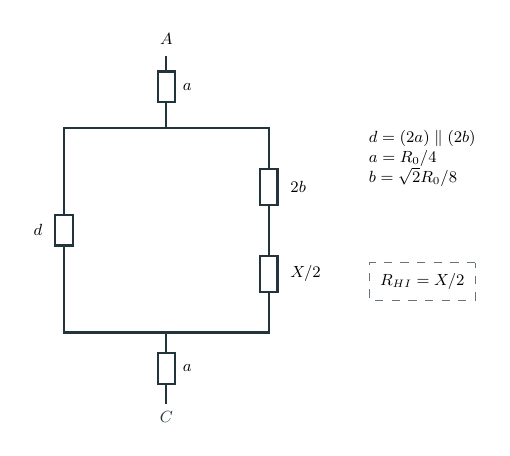
\begin{tikzpicture}[scale=.65,transform shape]

\node[above] at (0,4.5) {$A$};
\draw[object] (0,4.4)--(0,4.1);
\draw[object] (-.17,3.5) rectangle (.17,4.1);\node[right] at (.2,3.8) {$a$};
\draw[object] (0,3.5)--(0,3)--(-2,3)--(-2,1.3);
\draw[object] (-2.17,.7) rectangle (-1.83,1.3);\node[left] at (-2.3,1) {$d$};
\draw[object] (-2,.7)--(-2,-1)--(2,-1)--(2,-.2);
\draw[object] (1.83,-.2) rectangle (2.17,.5);\node[right] at (2.3,.15) {$X/2$};
\draw[object] (2,.5)--(2,1.5);
\draw[object] (1.83,1.5) rectangle (2.17,2.2);\node[right] at (2.3,1.85) {$2b$};
\draw[object] (2,2.2)--(2,3)--(0,3);
\draw[object] (0,-1)--(0,-1.4);
\draw[object] (-.17,-2) rectangle (.17,-1.4);\node[right] at (.2,-1.7) {$a$};
\draw[object] (0,-2)--(0,-2.4) node[below] {$C$};
\node[align=left] at (5,2.4) {$d=(2a)\parallel(2b)$\\$a=R_0/4$\\$b=\sqrt2R_0/8$};
\node[draw=muted,dashed,inner sep=6pt] at (5,0) {$R_{HI}=X/2$};

\end{tikzpicture}
\figcaption{解图电试3.2C\quad AC折叠等效中，内层同向对角线电阻为X的一半。}
\end{minipage}\end{center}
解图电试3.2C中，在两端串联的$a$之间，有两组并联通道：左侧外支路$2a$与中间支路$2b$先并联成$d$，右侧通道为$2b+R_{HI}$。$HI$相对于$AC$是隔两层的同向对角线，线性尺度减半，故$R_{HI}=X/2$。外层半边长对应$R_0/2$，折叠把左右两条这样的支路并联，得到$a=R_0/4$。第一内层边长是外层的$1/\sqrt2$，其半边再折叠给$b=R_0/(4\sqrt2)$。$HI$间内网络跨过两次缩放，端口方向重新与$AC$相同，因此整体电阻为$X/2$。先并联$2a$与$2b$得到$d$，再将它与$2b+X/2$并联，最后串联两端$a$。于是
\[
\boxed{X=2a+\frac{d(2b+X/2)}{d+2b+X/2}}.
\]
令$t=X/(2b)$，利用$a=\sqrt2b$、$d=2(2-\sqrt2)b$，化为
\[
t^2+(4-2\sqrt2)t-4\sqrt2=0.
\]
从递推式移去两端的$2a$，再乘并联分母，得到关于$X$的二次方程。归一化为$t=X/(2b)$后，常数项为负，说明两根异号；正电阻对应其中正的根。两根中只有正根可作电阻，故
\[
t=\sqrt6+\sqrt2-2,\qquad
\boxed{R_{AC}=\frac{\sqrt3+1-\sqrt2}{2}R_0}.
\]
递推右边对$X$的导数为
\[
\frac{d^2}{2(d+2b+X/2)^2}<\frac12\quad(X\ge0).
\]
所以不同有限层终端的影响逐层衰减，正固定点为有限截断网络的唯一极限，其数值由给定的有限截断定义唯一确定。
\begin{center}\begin{minipage}{.98\linewidth}\centering
\begin{tikzpicture}[scale=.85,transform shape]

\draw[object] (0,0)--(0,1.7)--(5,1.7)--(5,-1.7)--(0,-1.7)--(0,0);
\draw[object] (0,0)--(5,0);
\node[draw=ink,fill=white,minimum width=1.5cm,minimum height=.45cm] at (2.5,1.7) {$2R_0$};
\node[draw=ink,fill=white,minimum width=1.5cm,minimum height=.45cm] at (2.5,0) {$X/\sqrt2$};
\node[draw=ink,fill=white,minimum width=1.5cm,minimum height=.45cm] at (2.5,-1.7) {$2R_0$};
\draw[motion] (-1,0)--(-.1,0);\draw[motion] (5.1,0)--(6,0);
\node[above left] at (0,0) {$E$};\node[above right] at (5,0) {$G$};
\node at (2.5,2.6) {外圈通路、内侧网络、外圈通路并联};

\end{tikzpicture}
\figcaption{解图电试3.2D\quad EG端口的内侧与AC网络相似、尺度缩小一层，外围另有两条通路。}
\end{minipage}\end{center}
\begin{center}\begin{minipage}{.98\linewidth}\centering
\begin{tikzpicture}[scale=.8,transform shape]
\draw[axis] (0,0)--(10.7,0) node[right] {内接层数$N$};
\draw[axis] (0,0)--(0,3.2) node[above] {$R/R_0$};\foreach \y/\lab in {0/0,1.2/0.3,2.4/0.6}{\draw[thin] (0,\y)--(-.08,\y) node[left] {$\lab$};}
\node[above] at (5,3.5) {实线$AC$，虚线$EG$；有限层逐渐趋于无限极限};
\draw[traj] plot coordinates {(0.000000000,2.828427125) (0.909090909,2.666666667) (1.818181818,2.640754482) (2.727272727,2.636509763) (3.636363636,2.635811899) (4.545454545,2.635697097) (5.454545455,2.635678210) (6.363636364,2.635675102) (7.272727273,2.635674591) (8.181818182,2.635674507) (9.090909091,2.635674493) (10.000000000,2.635674491)};
\draw[dashed,thick,color=warm] plot coordinates {(0.000000000,1.656854249) (0.909090909,1.333333333) (1.818181818,1.281508964) (2.727272727,1.273019525) (3.636363636,1.271623799) (4.545454545,1.271394194) (5.454545455,1.271356420) (6.363636364,1.271350205) (7.272727273,1.271349182) (8.181818182,1.271349014) (9.090909091,1.271348986) (10.000000000,1.271348982)};
\node[below] at (0,-.12) {$1$};
\node[below] at (4.545454545454546,-.12) {$6$};
\node[below] at (10,-.12) {$12$};
\end{tikzpicture}
\figcaption{解图电试3.2E\quad 实线$AC$，虚线$EG$；有限层逐渐趋于无限极限}
\end{minipage}\end{center}
图E的每个有限层都在最内层保留完整正方形，且不再接入更深支路；两组曲线按相同截断方式得到。只保留外层时$R_{AC}^{(0)}=R_0$，保留第一内层时$R_{AC}^{(1)}=R_0/\sqrt2$。后续隔两层用同一递推更新，新增导线使端口电阻不增加，递推导数的上界则控制远端截断的影响，二者共同确定题设的无限极限。

再求$R_{EG}$。解图电试3.2D中，外层从$E$到$G$有两条各为$2R_0$的通路；内侧是以第一内接正方形为外边界的同类网络，$E,G$为其对角端点，电阻为$X/\sqrt2$。关于$FJ$反射会交换$E,G$，而$F,J$保持原位，故$F,J$均在两端平均电势上，各部分在这两点无净交换电流，可将这些等势结点拆开，三通道因而并联：
\[
\frac1{R_{EG}}=\frac1{2R_0}+\frac1{2R_0}
+\frac1{X/\sqrt2}
=\frac1{R_0}+\frac{\sqrt2}{X}.
\]
外侧两条路径分别经过外正方形上、右顶点与左、下顶点，每条包含四段半边，故电阻均为$2R_0$。内侧第一正方形的$E,G$是对角端口，线阻按其整体尺寸缩为$X/\sqrt2$。拆开$F,J$时，各子网络在这两个平均电势点的净交换电流为零，所以端口电流恰为三通道电流之和。代入$X$并有理化，
\[
\boxed{R_{EG}=(\sqrt3-\sqrt2)R_0}.
\]
两个结果都随$R_0$线性缩放；$R_{EG}<R_{AC}<R_0$也与可用通路和正电阻网络的单调性相符。


\Needspace{13\baselineskip}

\pdfbookmark[2]{第 3 题 双频理想电源驱动的稳态电流}{q3}

\section*{第 3 题\quad 双频理想电源驱动的稳态电流}\label{q:3}


两母线为$a,b$。理想电源$\mathcal E_1(t)=\mathcal E_0\sin^2\omega t$直接接于两母线，正方向使$V_a-V_b=\mathcal E_1$。上支路为电阻$R_2$与理想电源$\mathcal E_2(t)=\mathcal E_0\cos\omega t$串联，后者也以朝$a$方向升压为正。
中支路从$a$依次经过电感$L$，再通过并联的电容$C$和电阻$R_1$到$b$。已知
\[
R_1=R_2=R,\qquad L=\frac R{2\omega},\qquad
C=\frac1{2\omega R},
\]
电路已达到稳态。取流过$R_1$由左向右的电流为$i_1$，求$i_1(t)$并绘出曲线。说明$\mathcal E_2$是否影响$i_1$，以及稳态条件的作用。


\begin{center}\begin{minipage}{.98\linewidth}\centering
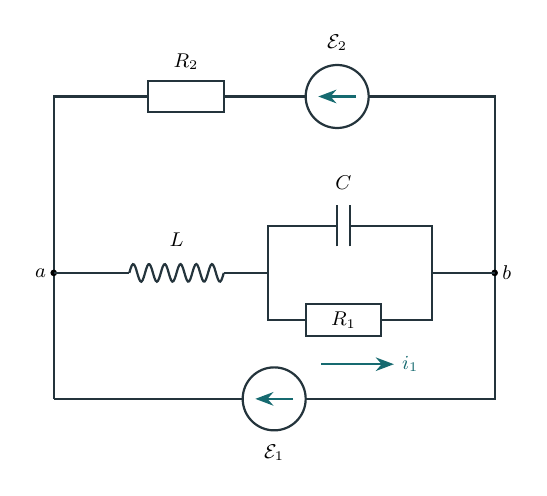
\begin{tikzpicture}[scale=.8,transform shape]

\draw[object] (0,-2)--(0,2.8)--(1.5,2.8);
\draw[object] (1.5,2.55) rectangle (2.7,3.05);
\draw[object] (2.7,2.8)--(4,2.8);
\draw[object] (4.5,2.8) circle (.5);
\draw[object] (5,2.8)--(7,2.8)--(7,-2)--(4,-2);
\draw[object] (3.5,-2) circle (.5);
\draw[object] (3,-2)--(0,-2);
\draw[motion] (3.8,-2)--(3.2,-2);
\draw[motion] (4.8,2.8)--(4.2,2.8);
\node[above] at (2.1,3.1) {$R_2$};
\node[above] at (4.5,3.4) {$\mathcal E_2$};
\node[below] at (3.5,-2.6) {$\mathcal E_1$};
\fill (0,0) circle (1.5pt) node[left] {$a$};
\fill (7,0) circle (1.5pt) node[right] {$b$};
\draw[object] (0,0)--(1.2,0);
\draw[object,domain=0:1.5,samples=80] plot ({1.2+\x},{.14*sin(1440*\x)});
\draw[object] (2.7,0)--(3.4,0)--(3.4,.75)--(4.5,.75);
\draw[object] (4.5,.42)--(4.5,1.08);\draw[object] (4.7,.42)--(4.7,1.08);
\draw[object] (4.7,.75)--(6,.75)--(6,-.75)--(5.2,-.75);
\draw[object] (4,-1) rectangle (5.2,-.5);
\draw[object] (4,-.75)--(3.4,-.75)--(3.4,0);
\draw[object] (6,0)--(7,0);
\node[above] at (1.95,.3) {$L$};
\node[above] at (4.6,1.2) {$C$};
\node at (4.6,-.75) {$R_1$};
\draw[motion] (4.25,-1.45)--(5.4,-1.45) node[right] {$i_1$};

\end{tikzpicture}
\figcaption{图电试3.3\quad 电源1直接固定母线电压，中支路为L串联电阻、电容的并联部分。}
\end{minipage}\end{center}

\Needspace{6\baselineskip}\subsection*{解答}


图电试3.3中理想电源$\mathcal E_1$直接规定两母线电压$V_a-V_b=\mathcal E_1$。令电阻、电容共同的端电压为$u$，其左端相对$b$为正，电感电流$i_L$取向右。并联结点的流入电流等于电阻电流与充电电流之和，电感压降再与$u$相加：
\[
i_L=\frac uR+C\dot u,\qquad
L\dot i_L+u=\mathcal E_1.
\]
消去$i_L$，得到中支路的时域方程
\[
\boxed{LC\ddot u+\frac LR\dot u+u=\mathcal E_1(t)}.
\]
上支路电源2改变电源1承担的电流；中支路的输入始终是已给定的母线电压。上支路从$a$到$b$的电流为$(\mathcal E_1-\mathcal E_2)/R_2$，电源1随之补足两支路所需电流；这一连接关系先于任何频率计算成立。

把母线输入分解为
\[
\mathcal E_1=\frac{\mathcal E_0}{2}
-\frac{\mathcal E_0}{2}\cos2\omega t.
\]
直流稳态中$\dot i_L=0$、$\dot u=0$，电感压降为零、电容无电流，相当于电感短路、电容断路，故
\[
u_{\rm dc}=\frac{\mathcal E_0}{2},\qquad
i_{1,\rm dc}=\frac{\mathcal E_0}{2R}.
\]
这一恒定电压构成最后曲线的平均基线。剩下的交流项单独在角频率$2\omega$下计算。
\begin{center}\begin{minipage}{.98\linewidth}\centering
\begin{tikzpicture}[scale=.75,transform shape]

\draw[object] (0,-.5) circle (.45);
\draw[motion] (0,-.75)--(0,-.25);
\node[left] at (-.6,-.5) {$\widetilde{\mathcal E}$};
\draw[object] (0,-.05)--(0,1)--(1.3,1);
\draw[object] (1.3,.75) rectangle (3.1,1.25);
\node[above] at (2.2,1.4) {$j\Omega L$};
\draw[object] (3.1,1)--(5,1)--(5,.2);
\draw[object] (4.7,-1.2) rectangle (5.3,.2);
\node at (5,-.5) {$Z_p$};
\draw[object] (5,-1.2)--(5,-2)--(0,-2)--(0,-.95);
\draw[axis,<->] (6,-1.7)--(6,.7) node[midway,right] {$\widetilde u$};
\node at (2.8,-3) {$Z_p=R/(1+j\Omega RC),\quad H(2\omega)=-j$};
\node at (2.8,2.4) {$2\omega$交流等效；直流分量另算};

\end{tikzpicture}
\figcaption{解图电试3.3A\quad 并联端电压是输出量，负余弦输入与传函相位同时计入。}
\end{minipage}\end{center}
对角频率$\Omega$的余弦分量采用$e^{j\Omega t}$约定。解图电试3.3A中的并联阻抗由电导相加给出，输出$\widetilde u$是该阻抗的端电压，因此
\[
Z_p=\frac{R}{1+j\Omega RC},\qquad
H(\Omega)=\frac{\widetilde u}{\widetilde{\mathcal E}}
=\frac{Z_p}{j\Omega L+Z_p}
=\frac1{1-\Omega^2LC+j\Omega L/R}.
\]
分母实部来自电感、电容的共同作用，虚部来自电阻电流对应的电感压降。题设$\Omega=2\omega$时，$2\omega L=R$、$1/(2\omega C)=R$，即电感电抗、电容电抗和电阻数值相等。
\begin{center}\begin{minipage}{.98\linewidth}\centering
\begin{tikzpicture}[scale=.8,transform shape]
\draw[axis] (0,0)--(4.3,0) node[right] {$\widetilde U_{RC}$};\draw[motion] (0,0)--(0,2) node[above left] {$\widetilde I_C$};\draw[motion] (0,0)--(2,0) node[below] {$\widetilde I_R$};\draw[motion] (0,0)--(2,2) node[above right] {$\widetilde I$};\draw[guide] (0,2)--(2,2)--(2,0);\draw[force] (0,0)--(-4,4) node[left] {$\widetilde U_L$};\draw[force] (0,0)--(0,4) node[above right] {$\widetilde U$};\draw[guide] (-4,4)--(0,4)--(4,0);\draw (0.7,0) arc(0:45:.7);\node at (1,.4) {$45^\circ$};\node[align=center] at (0,-1.2) {以正余弦辅助输入定向；电流与电压分别使用比例尺};
\end{tikzpicture}
\figcaption{解图电试3.3D\quad 并联相量与串联电压相加，实际负余弦分量再计入负号}
\end{minipage}\end{center}
解图电试3.3D先用正余弦辅助激励定相位，取$\widetilde U_{RC}$水平向右。电阻电流同向，电容电流超前$90^\circ$且幅值相等，所以$I=\sqrt2 I_R$、总电流沿$45^\circ$。电感电压再超前总电流$90^\circ$，其幅值$U_L=I(2\omega)L=\sqrt2 U_{RC}$，分量为$(-U_{RC},U_{RC})$。与并联电压$(U_{RC},0)$相加，输入电压恰沿竖直向上，幅值仍为$U_{RC}$；并联电压落后输入$90^\circ$。同一关系写成复数，就是$\Omega^2LC=1$、$\Omega L/R=1$时
\[
H(2\omega)=\frac1j=-j.
\]
实际交流输入为负余弦，复振幅是$-\mathcal E_0/2$。把它与上述传递系数相乘再取实部，
\[
\widetilde u_{\rm ac}
=(-j)\left(-\frac{\mathcal E_0}{2}\right)
=j\frac{\mathcal E_0}{2},\qquad
u_{\rm ac}=\Re\left[j\frac{\mathcal E_0}{2}e^{j2\omega t}\right]
=-\frac{\mathcal E_0}{2}\sin2\omega t.
\]
负余弦的复振幅为负实数，与传递相位一起决定输出的正负。正余弦辅助电路中$i_R=\mathcal E_0\sin2\omega t/(2R)$，实际分量则为$-i_R$；这与复振幅的乘法是同一步相位关系的两种表示。再叠加直流，得到
\[
\boxed{i_1(t)=\frac{\mathcal E_0}{2R}
\bigl(1-\sin2\omega t\bigr)}.
\]
\begin{center}\begin{minipage}{.98\linewidth}\centering
\begin{tikzpicture}[scale=.8,transform shape]
\draw[axis] (0,0)--(10.7,0) node[right] {$\omega t$};
\draw[axis] (0,0)--(0,3.2) node[above] {$i_1R/\mathcal E_0$};\foreach \y/\lab in {0/0,1.5/0.5,3/1}{\draw[thin] (0,\y)--(-.08,\y) node[left] {$\lab$};}
\node[above] at (5,3.5) {周期$\pi/\omega$，平均值$1/2$，先从平均线向下};
\draw[traj] plot coordinates {(0.000000000,1.500000000) (0.062500000,1.382311356) (0.125000000,1.265348302) (0.187500000,1.149831954) (0.250000000,1.036474508) (0.312500000,0.925974851) (0.375000000,0.819014250) (0.437500000,0.716252153) (0.500000000,0.618322122) (0.562500000,0.525827928) (0.625000000,0.439339828) (0.687500000,0.359391052) (0.750000000,0.286474508) (0.812500000,0.221039753) (0.875000000,0.163490214) (0.937500000,0.114180701) (1.000000000,0.073415226) (1.062500000,0.041445119) (1.125000000,0.018467489) (1.187500000,0.004623999) (1.250000000,0.000000000) (1.312500000,0.004623999) (1.375000000,0.018467489) (1.437500000,0.041445119) (1.500000000,0.073415226) (1.562500000,0.114180701) (1.625000000,0.163490214) (1.687500000,0.221039753) (1.750000000,0.286474508) (1.812500000,0.359391052) (1.875000000,0.439339828) (1.937500000,0.525827928) (2.000000000,0.618322122) (2.062500000,0.716252153) (2.125000000,0.819014250) (2.187500000,0.925974851) (2.250000000,1.036474508) (2.312500000,1.149831954) (2.375000000,1.265348302) (2.437500000,1.382311356) (2.500000000,1.500000000) (2.562500000,1.617688644) (2.625000000,1.734651698) (2.687500000,1.850168046) (2.750000000,1.963525492) (2.812500000,2.074025149) (2.875000000,2.180985750) (2.937500000,2.283747847) (3.000000000,2.381677878) (3.062500000,2.474172072) (3.125000000,2.560660172) (3.187500000,2.640608948) (3.250000000,2.713525492) (3.312500000,2.778960247) (3.375000000,2.836509786) (3.437500000,2.885819299) (3.500000000,2.926584774) (3.562500000,2.958554881) (3.625000000,2.981532511) (3.687500000,2.995376001) (3.750000000,3.000000000) (3.812500000,2.995376001) (3.875000000,2.981532511) (3.937500000,2.958554881) (4.000000000,2.926584774) (4.062500000,2.885819299) (4.125000000,2.836509786) (4.187500000,2.778960247) (4.250000000,2.713525492) (4.312500000,2.640608948) (4.375000000,2.560660172) (4.437500000,2.474172072) (4.500000000,2.381677878) (4.562500000,2.283747847) (4.625000000,2.180985750) (4.687500000,2.074025149) (4.750000000,1.963525492) (4.812500000,1.850168046) (4.875000000,1.734651698) (4.937500000,1.617688644) (5.000000000,1.500000000) (5.062500000,1.382311356) (5.125000000,1.265348302) (5.187500000,1.149831954) (5.250000000,1.036474508) (5.312500000,0.925974851) (5.375000000,0.819014250) (5.437500000,0.716252153) (5.500000000,0.618322122) (5.562500000,0.525827928) (5.625000000,0.439339828) (5.687500000,0.359391052) (5.750000000,0.286474508) (5.812500000,0.221039753) (5.875000000,0.163490214) (5.937500000,0.114180701) (6.000000000,0.073415226) (6.062500000,0.041445119) (6.125000000,0.018467489) (6.187500000,0.004623999) (6.250000000,0.000000000) (6.312500000,0.004623999) (6.375000000,0.018467489) (6.437500000,0.041445119) (6.500000000,0.073415226) (6.562500000,0.114180701) (6.625000000,0.163490214) (6.687500000,0.221039753) (6.750000000,0.286474508) (6.812500000,0.359391052) (6.875000000,0.439339828) (6.937500000,0.525827928) (7.000000000,0.618322122) (7.062500000,0.716252153) (7.125000000,0.819014250) (7.187500000,0.925974851) (7.250000000,1.036474508) (7.312500000,1.149831954) (7.375000000,1.265348302) (7.437500000,1.382311356) (7.500000000,1.500000000) (7.562500000,1.617688644) (7.625000000,1.734651698) (7.687500000,1.850168046) (7.750000000,1.963525492) (7.812500000,2.074025149) (7.875000000,2.180985750) (7.937500000,2.283747847) (8.000000000,2.381677878) (8.062500000,2.474172072) (8.125000000,2.560660172) (8.187500000,2.640608948) (8.250000000,2.713525492) (8.312500000,2.778960247) (8.375000000,2.836509786) (8.437500000,2.885819299) (8.500000000,2.926584774) (8.562500000,2.958554881) (8.625000000,2.981532511) (8.687500000,2.995376001) (8.750000000,3.000000000) (8.812500000,2.995376001) (8.875000000,2.981532511) (8.937500000,2.958554881) (9.000000000,2.926584774) (9.062500000,2.885819299) (9.125000000,2.836509786) (9.187500000,2.778960247) (9.250000000,2.713525492) (9.312500000,2.640608948) (9.375000000,2.560660172) (9.437500000,2.474172072) (9.500000000,2.381677878) (9.562500000,2.283747847) (9.625000000,2.180985750) (9.687500000,2.074025149) (9.750000000,1.963525492) (9.812500000,1.850168046) (9.875000000,1.734651698) (9.937500000,1.617688644) (10.000000000,1.500000000)};
\node[below] at (1.25,-.12) {$\pi/4$};
\node[below] at (3.75,-.12) {$3\pi/4$};
\node[below] at (6.25,-.12) {$5\pi/4$};
\node[below] at (8.75,-.12) {$7\pi/4$};
\end{tikzpicture}
\figcaption{解图电试3.3B\quad 周期$\pi/\omega$，平均值$1/2$，先从平均线向下}
\end{minipage}\end{center}
解图电试3.3B以$\omega t$为横坐标，电流用$\mathcal E_0/R$归一化。因为$\sin2\omega t$每经过$\pi/\omega$重复一次，电流周期为$\pi/\omega$，平均值为$\mathcal E_0/(2R)$，全程非负。极值为
\[
i_{1,\min}=0\quad
(\omega t=\pi/4+k\pi),\qquad
i_{1,\max}=\frac{\mathcal E_0}{R}\quad
(\omega t=3\pi/4+k\pi).
\]
在$t=0$，$i_1=\mathcal E_0/(2R)$且$\dot i_1=-\mathcal E_0\omega/R$；到$\omega t=\pi/4$降到零，再在$\pi/2$回到平均线向上，通过$3\pi/4$的最高点。曲线在平均线起步，先向下到达零点。

按电源叠加单独计算$\mathcal E_2$时，理想电源1置零成为连接$a,b$的导线。中支路的外加电压随之为零，周期稳态响应为零，故电源2对$i_1$的稳态贡献为$i(3)=0$。电源2仍可向上支路供能，其电流由电源1的短接支路回流。

稳态条件决定怎样处理初始储能。将给定参数代入齐次方程，
\[
\ddot u+2\omega\dot u+4\omega^2u=0,
\]
特征方程$s^2+2\omega s+4\omega^2=0$的根为$-\omega\pm j\sqrt3\,\omega$，所以一般响应在周期部分外还有
\[
u_h=e^{-\omega t}
\left(A\cos\sqrt3\,\omega t+B\sin\sqrt3\,\omega t\right).
\]
\begin{center}\begin{minipage}{.98\linewidth}\centering
\begin{tikzpicture}[scale=.8,transform shape]
\draw[axis] (0,0)--(10.7,0) node[right] {$\omega t$};
\draw[axis] (0,0)--(0,3.2) node[above] {$i_1R/\mathcal E_0$};\foreach \y/\lab in {0/0,1.4/0.5,2.8/1}{\draw[thin] (0,\y)--(-.08,\y) node[left] {$\lab$};}
\node[above] at (5,3.5) {实线：零储能接通；虚线：周期稳态};
\draw[traj] plot coordinates {(0.000000000,0.000000000) (0.071428571,0.000005715) (0.142857143,0.000089483) (0.214285714,0.000442854) (0.285714286,0.001366810) (0.357142857,0.003255194) (0.428571429,0.006577557) (0.500000000,0.011861707) (0.571428571,0.019676193) (0.642857143,0.030612968) (0.714285714,0.045270480) (0.785714286,0.064237366) (0.857142857,0.088076986) (0.928571429,0.117312938) (1.000000000,0.152415734) (1.071428571,0.193790771) (1.142857143,0.241767707) (1.214285714,0.296591346) (1.285714286,0.358414104) (1.357142857,0.427290109) (1.428571429,0.503170973) (1.500000000,0.585903239) (1.571428571,0.675227503) (1.642857143,0.770779182) (1.714285714,0.872090876) (1.785714286,0.978596268) (1.857142857,1.089635481) (1.928571429,1.204461788) (2.000000000,1.322249582) (2.071428571,1.442103469) (2.142857143,1.563068365) (2.214285714,1.684140448) (2.285714286,1.804278824) (2.357142857,1.922417745) (2.428571429,2.037479232) (2.500000000,2.148385938) (2.571428571,2.254074090) (2.642857143,2.353506353) (2.714285714,2.445684467) (2.785714286,2.529661493) (2.857142857,2.604553538) (2.928571429,2.669550806) (3.000000000,2.723927866) (3.071428571,2.767053002) (3.142857143,2.798396541) (3.214285714,2.817538079) (3.285714286,2.824172500) (3.357142857,2.818114741) (3.428571429,2.799303235) (3.500000000,2.767802008) (3.571428571,2.723801389) (3.642857143,2.667617337) (3.714285714,2.599689393) (3.785714286,2.520577267) (3.857142857,2.430956112) (3.928571429,2.331610520) (4.000000000,2.223427314) (4.071428571,2.107387214) (4.142857143,1.984555456) (4.214285714,1.856071474) (4.285714286,1.723137744) (4.357142857,1.587007921) (4.428571429,1.448974382) (4.500000000,1.310355308) (4.571428571,1.172481454) (4.642857143,1.036682723) (4.714285714,0.904274706) (4.785714286,0.776545320) (4.857142857,0.654741681) (4.928571429,0.540057353) (5.000000000,0.433620109) (5.071428571,0.336480326) (5.142857143,0.249600139) (5.214285714,0.173843461) (5.285714286,0.109966989) (5.357142857,0.058612266) (5.428571429,0.020298906) (5.500000000,-0.004580964) (5.571428571,-0.015766981) (5.642857143,-0.013133490) (5.714285714,0.003308866) (5.785714286,0.033412932) (5.857142857,0.076896212) (5.928571429,0.133343405) (6.000000000,0.202210290) (6.071428571,0.282828918) (6.142857143,0.374414058) (6.214285714,0.476070837) (6.285714286,0.586803497) (6.357142857,0.705525177) (6.428571429,0.831068629) (6.500000000,0.962197750) (6.571428571,1.097619829) (6.642857143,1.235998370) (6.714285714,1.375966374) (6.785714286,1.516139941) (6.857142857,1.655132055) (6.928571429,1.791566415) (7.000000000,1.924091171) (7.071428571,2.051392431) (7.142857143,2.172207392) (7.214285714,2.285336980) (7.285714286,2.389657855) (7.357142857,2.484133668) (7.428571429,2.567825459) (7.500000000,2.639901080) (7.571428571,2.699643563) (7.642857143,2.746458339) (7.714285714,2.779879232) (7.785714286,2.799573177) (7.857142857,2.805343607) (7.928571429,2.797132482) (8.000000000,2.775020922) (8.071428571,2.739228461) (8.142857143,2.690110912) (8.214285714,2.628156865) (8.285714286,2.553982867) (8.357142857,2.468327306) (8.428571429,2.372043090) (8.500000000,2.266089169) (8.571428571,2.151520996) (8.642857143,2.029480029) (8.714285714,1.901182355) (8.785714286,1.767906580) (8.857142857,1.630981083) (8.928571429,1.491770772) (9.000000000,1.351663467) (9.071428571,1.212056059) (9.142857143,1.074340572) (9.214285714,0.939890266) (9.285714286,0.810045931) (9.357142857,0.686102499) (9.428571429,0.569296114) (9.500000000,0.460791786) (9.571428571,0.361671752) (9.642857143,0.272924667) (9.714285714,0.195435721) (9.785714286,0.129977794) (9.857142857,0.077203729) (9.928571429,0.037639806) (10.000000000,0.011680474)};
\draw[dashed,thick,color=warm] plot coordinates {(0.000000000,1.400000000) (0.071428571,1.260233217) (0.142857143,1.121862937) (0.214285714,0.986271711) (0.285714286,0.854814321) (0.357142857,0.728804246) (0.428571429,0.609500537) (0.500000000,0.498095238) (0.571428571,0.395701473) (0.642857143,0.303342327) (0.714285714,0.221940621) (0.785714286,0.152309696) (0.857142857,0.095145280) (0.928571429,0.051018540) (1.000000000,0.020370378) (1.071428571,0.003507019) (1.142857143,0.000596956) (1.214285714,0.011669265) (1.285714286,0.036613317) (1.357142857,0.075179877) (1.428571429,0.126983602) (1.500000000,0.191506887) (1.571428571,0.268105035) (1.642857143,0.356012703) (1.714285714,0.454351547) (1.785714286,0.562138998) (1.857142857,0.678298079) (1.928571429,0.801668168) (2.000000000,0.931016590) (2.071428571,1.065050939) (2.142857143,1.202431989) (2.214285714,1.341787073) (2.285714286,1.481723801) (2.357142857,1.620843972) (2.428571429,1.757757543) (2.500000000,1.891096519) (2.571428571,2.019528621) (2.642857143,2.141770597) (2.714285714,2.256601047) (2.785714286,2.362872623) (2.857142857,2.459523493) (2.928571429,2.545587955) (3.000000000,2.620206081) (3.071428571,2.682632311) (3.142857143,2.732242903) (3.214285714,2.768542165) (3.285714286,2.791167405) (3.357142857,2.799892561) (3.428571429,2.794630452) (3.500000000,2.775433658) (3.571428571,2.742493985) (3.642857143,2.696140555) (3.714285714,2.636836518) (3.785714286,2.565174419) (3.857142857,2.481870283) (3.928571429,2.387756456) (4.000000000,2.283773293) (4.071428571,2.170959760) (4.142857143,2.050443051) (4.214285714,1.923427331) (4.285714286,1.791181697) (4.357142857,1.655027506) (4.428571429,1.516325164) (4.500000000,1.376460539) (4.571428571,1.236831113) (4.642857143,1.098832017) (4.714285714,0.963842091) (4.785714286,0.833210111) (4.857142857,0.708241308) (4.928571429,0.590184330) (5.000000000,0.480218762) (5.071428571,0.379443344) (5.142857143,0.288864991) (5.214285714,0.209388731) (5.285714286,0.141808666) (5.357142857,0.086800033) (5.428571429,0.044912459) (5.500000000,0.016564473) (5.571428571,0.002039316) (5.642857143,0.001482121) (5.714285714,0.014898455) (5.785714286,0.042154265) (5.857142857,0.082977221) (5.928571429,0.136959433) (6.000000000,0.203561529) (6.071428571,0.282118042) (6.142857143,0.371844063) (6.214285714,0.471843078) (6.285714286,0.581115930) (6.357142857,0.698570801) (6.428571429,0.823034121) (6.500000000,0.953262293) (6.571428571,1.087954120) (6.642857143,1.225763807) (6.714285714,1.365314404) (6.785714286,1.505211569) (6.857142857,1.644057494) (6.928571429,1.780464877) (7.000000000,1.913070781) (7.071428571,2.040550251) (7.142857143,2.161629555) (7.214285714,2.275098908) (7.285714286,2.379824563) (7.357142857,2.474760134) (7.428571429,2.558957057) (7.500000000,2.631574064) (7.571428571,2.691885590) (7.642857143,2.739289023) (7.714285714,2.773310722) (7.785714286,2.793610755) (7.857142857,2.799986289) (7.928571429,2.792373623) (8.000000000,2.770848821) (8.071428571,2.735626950) (8.142857143,2.687059936) (8.214285714,2.625633045) (8.285714286,2.551960033) (8.357142857,2.466777017) (8.428571429,2.370935119) (8.500000000,2.265391957) (8.571428571,2.151202085) (8.642857143,2.029506450) (8.714285714,1.901520995) (8.785714286,1.768524508) (8.857142857,1.631845846) (8.928571429,1.492850656) (9.000000000,1.352927734) (9.071428571,1.213475142) (9.142857143,1.075886245) (9.214285714,0.941535785) (9.285714286,0.811766148) (9.357142857,0.687873950) (9.428571429,0.571097079) (9.500000000,0.462602333) (9.571428571,0.363473754) (9.642857143,0.274701803) (9.714285714,0.197173459) (9.785714286,0.131663361) (9.857142857,0.078826063) (9.928571429,0.039189498) (10.000000000,0.013149702)};
\node[below] at (0,-.12) {$0$};
\node[below] at (5,-.12) {$3.5$};
\node[below] at (10,-.12) {$7$};
\end{tikzpicture}
\figcaption{解图电试3.3C\quad 实线：零储能接通；虚线：周期稳态}
\end{minipage}\end{center}
解图电试3.3C取同一输入从$t=0$接通，电容电压和电感电流均从零开始作比较。此时$u(0)=0$，结点式给$\dot u(0)=0$，而周期解在零时刻分别为$\mathcal E_0/2$、$-\mathcal E_0\omega$；两者之差确定$A=-\mathcal E_0/2$、$B=\mathcal E_0/(2\sqrt3)$。指数因子使差值在时间尺度$1/\omega$上衰减。题设已达到稳定状态，保留的是图B的周期部分。理想电源规定端电压，初始储能形成图C中的衰减分量，其幅值由接通时的电压和电流确定。



\Needspace{13\baselineskip}

\pdfbookmark[2]{第 4 题 三棱柱交流网络与最小补偿电容}{q4}

\section*{第 4 题\quad 三棱柱交流网络与最小补偿电容}\label{q:4}


三棱柱的上三角形为$ABC$、下三角形为$EDF$，对应连接棱为$AE,BD,CF$。九条棱各为相同的电阻$R$与电感$L$串联支路。给定角频率$\omega$下，$\omega L=\sqrt3R$。
\begin{enumerate}
\item 求$A,B$间等效复阻抗的模，答案用$R$表示。
\item 以$A,D$为输入输出端，在每一条支路中串联相同电容$C_1$，使整个网络功率因数为$1/\sqrt2$。求最小$C_1$。
\item 各支路不加电容，仅在网络$AD$外串一个电容$C_2$，使总串联组合功率因数为$1/\sqrt2$，求最小$C_2$。
\end{enumerate}
求最小值时须比较总无功为感性和容性两种可能。


\begin{center}\begin{minipage}{.98\linewidth}\centering
\begin{tikzpicture}[scale=.75,transform shape]

\coordinate (A) at (0,2.8);\coordinate (B) at (3.4,2.8);\coordinate (C) at (1.7,4.5);
\coordinate (E) at (0,0);\coordinate (D) at (3.4,0);\coordinate (F) at (1.7,1.7);
\draw[object] (A)--(B)--(C)--cycle;
\draw[object] (A)--(E)--(D)--(B);
\draw[guide] (E)--(F)--(D);\draw[guide] (C)--(F);
\foreach \p/\pos in {A/above left,B/right,C/above,D/below right,E/left,F/above left}
{\fill (\p) circle (1.5pt);\node[\pos] at (\p) {$\p$};}

\node[align=left] at (7,3) {九条棱各为串联$R,L$\\$z=R+j\sqrt3R$\\$|z|=2R$};
\node[align=left] at (7,.8) {端口一：$A,B$\\端口二：$A,D$};

\end{tikzpicture}
\figcaption{图电试3.4\quad 三棱柱的虚线棱也实际导电，端口选择决定等势结点。}
\end{minipage}\end{center}

\Needspace{6\baselineskip}\subsection*{解答}


图电试3.4的九支路阻抗均为
\[
z=R+j\omega L=R(1+j\sqrt3),\qquad |z|=2R.
\]
因为所有支路都是同一个$z$，结点方程可整体约去$1/z$，所以任何指定端口的等效阻抗都等于一个只由拓扑决定的正实系数乘$z$。支路电流的相位由共同复阻抗决定，拓扑约化只处理各支路的实数比例。

具体地，对任一未接电源的结点有$\sum_j(V_i-V_j)/z=0$，约去共同的$1/z$后，只剩连接图的实系数方程。给定总复电流时，电势可写成$\widetilde Iz$乘实数，端口电势差也如此，因此所有拓扑化简均保留复阻抗因子。

第（1）问从$A$入、$B$出时，对称性使$C,F$都在端口平均电势上，交换$A,B$及$E,D$而保持$C,F$不动的反射使电势变成端口电势和减自身，故$V_C=V_F=(V_A+V_B)/2$。连接棱$CF$无电流，可以移除。
\begin{center}\begin{minipage}{.98\linewidth}\centering
\begin{tikzpicture}[scale=.8,transform shape]

\draw[object] (0,0)--(0,2)--(4,2)--(4,0)--cycle;
\node[fill=white] at (2,2) {$2z/3$};
\node[fill=white] at (2,0) {$2z/3$};
\node[fill=white] at (0,1) {$z$};\node[fill=white] at (4,1) {$z$};
\node[above left] at (0,2) {$A$};\node[above right] at (4,2) {$B$};
\node[below left] at (0,0) {$E$};\node[below right] at (4,0) {$D$};
\node[align=center] at (7,1) {$C,F$等势\\$CF$无电流\\两通路并联};
\node at (3.4,-1) {上支路$2z/3$，下绕行支路$8z/3$};

\end{tikzpicture}
\figcaption{解图电试3.4A\quad AB端口下删去零电流棱，各三角形的直接与绕行支路先并联。}
\end{minipage}\end{center}
解图电试3.4A中，上三角形$AB$间的直接支路$z$与经$C$的$2z$并联为$2z/3$；下三角形$ED$间同样化为$2z/3$。端口$AB$还可沿$A\to E\to D\to B$经过串联阻抗$z+2z/3+z=8z/3$，两条通路并联：
\[
\widetilde Z_{AB}
=\frac{2z}{3}\parallel\frac{8z}{3}
=\frac8{15}z.
\]
因此
\[
\boxed{|\widetilde Z_{AB}|=\frac8{15}(2R)
=\frac{16}{15}R}.
\]
$8R/15$为等效有功电阻；题问要求的阻抗模还包含电感电抗，数值为$16R/15$。

第（2）问每支路同加一个$C_1$后，支路阻抗仍处处相同：
\[
z_1=R+j\left(\sqrt3R-\frac1{\omega C_1}\right).
\]
此时整个$AD$阻抗为$kz_1$，$k>0$。功率因数$\Re(kz_1)/|kz_1|$中$k$相消，所以本问可先按每一支路确定相位，故功率因数为
\[
\frac R{\sqrt{R^2+(\sqrt3R-1/\omega C_1)^2}}
=\frac1{\sqrt2}.
\]
\begin{center}\begin{minipage}{.98\linewidth}\centering
\begin{tikzpicture}[scale=.8,transform shape]
\draw[axis] (0,-2.5)--(0,4.3) node[above] {$X/R$};\draw[axis] (0,0)--(5.2,0) node[right] {$\Re z/R$};\draw[guide] (2,-2.2)--(2,3.8);\draw[motion] (0,0)--(2,3.464101615) node[above right] {未补偿$\sqrt3$};\draw[force] (0,0)--(2,2) node[right] {$+1$};\draw[force] (0,0)--(2,-2) node[right] {$-1$};\draw[axis] (4.3,3.3)--(4.3,-1.9) node[midway,right] {容抗增加};\node[below] at (2,0) {$1$};\node at (1.7,-3.2) {横纵同尺度，容性目标所需容抗更大};
\end{tikzpicture}
\figcaption{解图电试3.4B\quad 电抗从正值沿竖直方向降低，两个目标对应相同功率因数}
\end{minipage}\end{center}
从图B中起点的电抗$\sqrt3R$向下移动，功率因数$1/\sqrt2$要求$R^2+X^2=2R^2$。相同的相位余弦对应上下两个目标点，解图电试3.4B中的竖直电抗可以为$+R$或$-R$，于是
\[
\sqrt3R-\frac1{\omega C_1}=\pm R,\qquad
C_1=\frac1{\omega R(\sqrt3\mp1)}.
\]
两个电容都为正，较小者对应电容补偿超过谐振、总支路为容性：
\[
\boxed{C_{1,\min}
=\frac1{(\sqrt3+1)\omega R}}.
\]
总电抗仍为感性的另一个解为$1/[(\sqrt3-1)\omega R]$，它大于容性解，两支正电容比较后选取上式。

第（3）问外接电容前，先求$AD$端口本身的拓扑系数。令总电流复振幅为$\widetilde I$，以从$A$到$E$的电流为$\widetilde I_1$，从$A$到$B$为$\widetilde I_2$。由交换$A,D$且同时交换$B,E$的端口反射对称，$BD$电流也为$\widetilde I_1$，$ED$电流也为$\widetilde I_2$。再由结点守恒，
\[
I_{AC}=I_{FD}=\widetilde I-\widetilde I_1-\widetilde I_2,\quad
I_{CB}=I_{EF}=\widetilde I_1-\widetilde I_2,\quad
I_{CF}=\widetilde I-2\widetilde I_1.
\]
本行各$I$均为复振幅，符号下标规定方向。
\begin{center}\begin{minipage}{.98\linewidth}\centering
\begin{tikzpicture}[scale=.65,transform shape]

\coordinate (A) at (0,2.8);\coordinate (B) at (3.4,2.8);\coordinate (C) at (1.7,4.5);
\coordinate (E) at (0,0);\coordinate (D) at (3.4,0);\coordinate (F) at (1.7,1.7);
\draw[object] (A)--(B)--(C)--cycle;
\draw[object] (A)--(E)--(D)--(B);
\draw[guide] (E)--(F)--(D);\draw[guide] (C)--(F);
\foreach \p/\pos in {A/above left,B/right,C/above,D/below right,E/left,F/above left}
{\fill (\p) circle (1.5pt);\node[\pos] at (\p) {$\p$};}

\draw[motion] (-1,2.8)--(-.1,2.8) node[midway,above] {$\widetilde I$};
\draw[motion] (3.5,0)--(4.4,0) node[midway,below] {$\widetilde I$};
\draw[motion] (0,2.4)--(0,1.3) node[midway,left] {$\widetilde I_1$};
\draw[motion] (.4,2.8)--(2.7,2.8) node[midway,below] {$\widetilde I_2$};
\draw[motion] (3.4,2.4)--(3.4,1.3) node[midway,right] {$\widetilde I_1$};
\draw[motion] (.4,0)--(2.7,0) node[midway,below] {$\widetilde I_2$};
\draw[force] (1.7,3.8)--(1.7,2);
\node[right,color=warm] at (1.8,2.2) {$I_{CF}$};
\node[align=left] at (7.3,3.4) {$I_{AC}=I_{FD}=I-I_1-I_2$\\$I_{CB}=I_{EF}=I_1-I_2$\\$I_{CF}=I-2I_1$\\本图各电流均为复振幅};
\node[align=left] at (7.3,1.1) {比较路径：$ACB$与$AB$\\比较路径：$ACF$与$AEF$};

\end{tikzpicture}
\figcaption{解图电试3.4C\quad AD端口保留CF电流，由结点守恒及两组路径电压求出比例。}
\end{minipage}\end{center}
解图电试3.4C按这些方向标出支路电流。比较$ACB$与$AB$的电压，
\[
(\widetilde I-\widetilde I_1-\widetilde I_2)z
+(\widetilde I_1-\widetilde I_2)z
=\widetilde I_2z,
\]
公共$z$约去后，左端为$\widetilde I-2\widetilde I_2$，故$\widetilde I=3\widetilde I_2$，得到$\widetilde I_2=\widetilde I/3$。再比较$ACF$与$AEF$，
\[
(\widetilde I-\widetilde I_1-\widetilde I_2)z
+(\widetilde I-2\widetilde I_1)z
=\widetilde I_1z+(\widetilde I_1-\widetilde I_2)z,
\]
同样约去$z$，左端为$2\widetilde I-3\widetilde I_1-\widetilde I_2$，右端为$2\widetilde I_1-\widetilde I_2$，因此$2\widetilde I=5\widetilde I_1$，得到$\widetilde I_1=2\widetilde I/5$。于是$AC,FD$各为$4\widetilde I/15$，$CB,EF$各为$\widetilde I/15$，$CF$为$\widetilde I/5$，方向均与图C一致。因此
\[
\widetilde U_{AD}=(\widetilde I_1+\widetilde I_2)z
=\frac{11}{15}\widetilde I z,\qquad
\boxed{\widetilde Z_{AD}=\frac{11}{15}z}.
\]
外串$C_2$后总阻抗为
\[
\widetilde Z_{\rm total}
=\frac{11R}{15}
+j\left(\frac{11\sqrt3R}{15}-\frac1{\omega C_2}\right).
\]
这里电容位于整个$AD$网络外部，其容抗只减一次，而网络的实部和电感电抗均先乘$11/15$。功率因数$1/\sqrt2$要求虚部等于实部的$\pm1$倍，故
\[
\frac1{\omega C_2}
=\frac{11R}{15}(\sqrt3\mp1).
\]
取更大的分母得到最小电容，
\[
\boxed{C_{2,\min}
=\frac{15}{11(\sqrt3+1)\omega R}
=\frac{15}{11}C_{1,\min}}.
\]
两种补偿的结果通过$AD$端口系数关联；前者在全部支路各串联一个电容，后者在整个网络外串联一个电容；外串补偿的容抗乘$11/15$，相应电容乘其倒数$15/11$。


\Needspace{13\baselineskip}

\pdfbookmark[2]{第 5 题 锯齿电源驱动的RC逐周期暂态}{q5}

\section*{第 5 题\quad 锯齿电源驱动的RC逐周期暂态}\label{q:5}


理想电容$C$、电阻$R$、开关$K$和理想电源串联，开始开路且电容不带电。$t=0$闭合开关。电源电动势周期为$T=RC$，在第$n$个完整周期内按
\[
\mathcal E(t)=\mathcal E_0\frac{t-nT}{T},
\qquad nT\le t<(n+1)T,\quad n=0,1,2,\ldots
\]
从零线性升至$\mathcal E_0$，到周期边界瞬间复位至零。
以$Q(t)$表示约定正极板上的带符号电荷，求$Q_N=Q(NT)$、$N=1,2,\ldots$及其$N\to\infty$的极限。给出任一周期内的电荷，并说明电源跳变时哪些量连续、连续时间解最终趋向何种状态。


\begin{center}\begin{minipage}{.98\linewidth}\centering
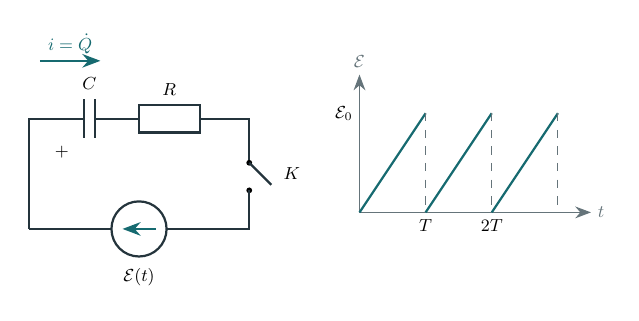
\begin{tikzpicture}[scale=.7,transform shape]

\draw[object] (0,0)--(0,2)--(1,2);
\draw[object] (1,1.65)--(1,2.35);\draw[object] (1.2,1.65)--(1.2,2.35);
\draw[object] (1.2,2)--(2,2);\draw[object] (2,1.75) rectangle (3.1,2.25);
\draw[object] (3.1,2)--(4,2)--(4,1.2);
\fill (4,1.2) circle (1.5pt);\fill (4,.7) circle (1.5pt);
\draw[object] (4,1.2)--(4.4,.8);\draw[object] (4,.7)--(4,0)--(2.5,0);
\draw[object] (2,0) circle (.5);\draw[object] (1.5,0)--(0,0);
\draw[motion] (2.3,0)--(1.7,0);
\node[above] at (1.1,2.4) {$C$};
\node[above] at (2.55,2.3) {$R$};
\node[right] at (4.5,1) {$K$};\node[below] at (2,-.6) {$\mathcal E(t)$};
\node at (.6,1.4) {$+$};\draw[motion] (.2,3.05)--(1.3,3.05) node[midway,above] {$i=\dot Q$};
\begin{scope}[xshift=6cm,yshift=.3cm]
\draw[axis] (0,0)--(4.2,0) node[right] {$t$};
\draw[axis] (0,0)--(0,2.5) node[above] {$\mathcal E$};
\foreach \n in {0,1,2}{\draw[traj] (\n*1.2,0)--({(\n+1)*1.2},1.8);
\draw[guide] ({(\n+1)*1.2},1.8)--({(\n+1)*1.2},0);}
\node[left] at (0,1.8) {$\mathcal E_0$};
\node[below] at (1.2,0) {$T$};\node[below] at (2.4,0) {$2T$};
\end{scope}

\end{tikzpicture}
\figcaption{图电试3.5\quad 电源在每个周期边界复位，正极板电荷由有限RC电流改变。}
\end{minipage}\end{center}

\Needspace{6\baselineskip}\subsection*{解答}


图电试3.5中取给电容正极板充电的方向为电流正方向，$i=\dot Q$。回路方程为
\[
Ri+\frac QC=\mathcal E(t),\qquad
\boxed{\dot Q+\frac Q{RC}=\frac{\mathcal E(t)}R}.
\]
电源电动势有限跳变时，电阻限制电流为有限值，故电容电荷与电压连续，$Q(NT^-)=Q(NT^+)$。电流随新回路电压有限跳变，电容电压则保留复位前的数值。

先算第一周期。利用$T=RC$，
\[
\dot Q+\frac QT=\frac{C\mathcal E_0}{T^2}t.
\]
乘积分因子$e^{t/T}$，
\[
\frac d{dt}(Qe^{t/T})
=\frac{C\mathcal E_0}{T^2}t e^{t/T}.
\]
由于
\[
\int t e^{t/T}dt=T(t-T)e^{t/T},
\]
因此积分后$Q=C\mathcal E_0(t/T-1)+Ae^{-t/T}$。在$t=0$，右端为$-C\mathcal E_0+A$，结合$Q(0)=0$求得$A=C\mathcal E_0$，得到
\[
\boxed{Q(t)=C\mathcal E_0\left(\frac tT-1+e^{-t/T}\right)}
\quad(0\le t<T),\qquad
Q_1=\frac{C\mathcal E_0}{e}.
\]
\begin{center}\begin{minipage}{.98\linewidth}\centering
\begin{tikzpicture}[scale=.8,transform shape]
\draw[axis] (0,0)--(10.7,0) node[right] {$t/T$};
\draw[axis] (0,0)--(0,3.2) node[above] {$Q/(C\mathcal E_0)$};\foreach \y/\lab in {0/0,1.4/0.5,2.8/1}{\draw[thin] (0,\y)--(-.08,\y) node[left] {$\lab$};}
\node[above] at (5,3.5) {电荷连续；虚线为同刻电源$\mathcal E/\mathcal E_0$};
\draw[traj] plot coordinates {(0.000000000,0.000000000) (0.031250000,0.000217841) (0.062500000,0.000867754) (0.093750000,0.001944370) (0.125000000,0.003442389) (0.156250000,0.005356576) (0.187500000,0.007681762) (0.218750000,0.010412841) (0.250000000,0.013544771) (0.281250000,0.017072572) (0.312500000,0.020991327) (0.343750000,0.025296180) (0.375000000,0.029982334) (0.406250000,0.035045053) (0.437500000,0.040479658) (0.468750000,0.046281531) (0.500000000,0.052446109) (0.531250000,0.058968886) (0.562500000,0.065845413) (0.593750000,0.073071295) (0.625000000,0.080642193) (0.656250000,0.088553820) (0.687500000,0.096801945) (0.718750000,0.105382387) (0.750000000,0.114291018) (0.781250000,0.123523761) (0.812500000,0.133076590) (0.843750000,0.142945529) (0.875000000,0.153126651) (0.906250000,0.163616078) (0.937500000,0.174409981) (0.968750000,0.185504576) (1.000000000,0.196896129) (1.031250000,0.208580951) (1.062500000,0.220555398) (1.093750000,0.232815874) (1.125000000,0.245358825) (1.156250000,0.258180741) (1.187500000,0.271278158) (1.218750000,0.284647653) (1.250000000,0.298285847) (1.281250000,0.312189402) (1.312500000,0.326355020) (1.343750000,0.340779448) (1.375000000,0.355459469) (1.406250000,0.370391909) (1.437500000,0.385573633) (1.468750000,0.401001543) (1.500000000,0.416672581) (1.531250000,0.432583728) (1.562500000,0.448732000) (1.593750000,0.465114452) (1.625000000,0.481728175) (1.656250000,0.498570296) (1.687500000,0.515637978) (1.718750000,0.532928418) (1.750000000,0.550438851) (1.781250000,0.568166542) (1.812500000,0.586108793) (1.843750000,0.604262939) (1.875000000,0.622626348) (1.906250000,0.641196419) (1.937500000,0.659970587) (1.968750000,0.678946315) (2.000000000,0.698121100) (2.031250000,0.717492468) (2.062500000,0.737057979) (2.093750000,0.756815220) (2.125000000,0.776761809) (2.156250000,0.796895395) (2.187500000,0.817213655) (2.218750000,0.837714294) (2.250000000,0.858395047) (2.281250000,0.879253677) (2.312500000,0.900287973) (2.343750000,0.921495755) (2.375000000,0.942874866) (2.406250000,0.964423178) (2.437500000,0.986138590) (2.468750000,1.008019026) (2.500000000,1.030062435) (2.531250000,1.017484636) (2.562500000,1.005497857) (2.593750000,0.994094757) (2.625000000,0.983268086) (2.656250000,0.973010683) (2.687500000,0.963315477) (2.718750000,0.954175483) (2.750000000,0.945583805) (2.781250000,0.937533631) (2.812500000,0.930018236) (2.843750000,0.923030975) (2.875000000,0.916565288) (2.906250000,0.910614697) (2.937500000,0.905172801) (2.968750000,0.900233283) (3.000000000,0.895789902) (3.031250000,0.891836494) (3.062500000,0.888366973) (3.093750000,0.885375329) (3.125000000,0.882855624) (3.156250000,0.880801996) (3.187500000,0.879208656) (3.218750000,0.878069886) (3.250000000,0.877380038) (3.281250000,0.877133537) (3.312500000,0.877324876) (3.343750000,0.877948614) (3.375000000,0.878999381) (3.406250000,0.880471872) (3.437500000,0.882360849) (3.468750000,0.884661137) (3.500000000,0.887367628) (3.531250000,0.890475275) (3.562500000,0.893979095) (3.593750000,0.897874167) (3.625000000,0.902155631) (3.656250000,0.906818687) (3.687500000,0.911858594) (3.718750000,0.917270671) (3.750000000,0.923050296) (3.781250000,0.929192901) (3.812500000,0.935693979) (3.843750000,0.942549077) (3.875000000,0.949753796) (3.906250000,0.957303793) (3.937500000,0.965194780) (3.968750000,0.973422521) (4.000000000,0.981982831) (4.031250000,0.990871581) (4.062500000,1.000084690) (4.093750000,1.009618129) (4.125000000,1.019467919) (4.156250000,1.029630130) (4.187500000,1.040100880) (4.218750000,1.050876338) (4.250000000,1.061952718) (4.281250000,1.073326282) (4.312500000,1.084993338) (4.343750000,1.096950241) (4.375000000,1.109193389) (4.406250000,1.121719228) (4.437500000,1.134524245) (4.468750000,1.147604973) (4.500000000,1.160957987) (4.531250000,1.174579903) (4.562500000,1.188467382) (4.593750000,1.202617126) (4.625000000,1.217025875) (4.656250000,1.231690413) (4.687500000,1.246607562) (4.718750000,1.261774185) (4.750000000,1.277187181) (4.781250000,1.292843491) (4.812500000,1.308740093) (4.843750000,1.324874000) (4.875000000,1.341242266) (4.906250000,1.357841979) (4.937500000,1.374670264) (4.968750000,1.391724282) (5.000000000,1.409001228) (5.031250000,1.391716175) (5.062500000,1.375080618) (5.093750000,1.359086487) (5.125000000,1.343725816) (5.156250000,1.328990735) (5.187500000,1.314873474) (5.218750000,1.301366356) (5.250000000,1.288461804) (5.281250000,1.276152332) (5.312500000,1.264430547) (5.343750000,1.253289150) (5.375000000,1.242720930) (5.406250000,1.232718768) (5.437500000,1.223275632) (5.468750000,1.214384577) (5.500000000,1.206038745) (5.531250000,1.198231365) (5.562500000,1.190955746) (5.593750000,1.184205283) (5.625000000,1.177973453) (5.656250000,1.172253812) (5.687500000,1.167040000) (5.718750000,1.162325731) (5.750000000,1.158104801) (5.781250000,1.154371081) (5.812500000,1.151118519) (5.843750000,1.148341138) (5.875000000,1.146033035) (5.906250000,1.144188381) (5.937500000,1.142801419) (5.968750000,1.141866462) (6.000000000,1.141377897) (6.031250000,1.141330178) (6.062500000,1.141717829) (6.093750000,1.142535441) (6.125000000,1.143777673) (6.156250000,1.145439252) (6.187500000,1.147514967) (6.218750000,1.149999673) (6.250000000,1.152888292) (6.281250000,1.156175804) (6.312500000,1.159857255) (6.343750000,1.163927752) (6.375000000,1.168382461) (6.406250000,1.173216609) (6.437500000,1.178425484) (6.468750000,1.184004430) (6.500000000,1.189948850) (6.531250000,1.196254205) (6.562500000,1.202916010) (6.593750000,1.209929838) (6.625000000,1.217291316) (6.656250000,1.224996125) (6.687500000,1.233040000) (6.718750000,1.241418729) (6.750000000,1.250128154) (6.781250000,1.259164165) (6.812500000,1.268522706) (6.843750000,1.278199770) (6.875000000,1.288191401) (6.906250000,1.298493690) (6.937500000,1.309102780) (6.968750000,1.320014859) (7.000000000,1.331226162) (7.031250000,1.342732973) (7.062500000,1.354531622) (7.093750000,1.366618482) (7.125000000,1.378989974) (7.156250000,1.391642561) (7.187500000,1.404572753) (7.218750000,1.417777100) (7.250000000,1.431252197) (7.281250000,1.444994681) (7.312500000,1.459001230) (7.343750000,1.473268564) (7.375000000,1.487793443) (7.406250000,1.502572668) (7.437500000,1.517603079) (7.468750000,1.532881557) (7.500000000,1.548405020) (7.531250000,1.529388265) (7.562500000,1.511042517) (7.593750000,1.493359441) (7.625000000,1.476330804) (7.656250000,1.459948478) (7.687500000,1.444204433) (7.718750000,1.429090741) (7.750000000,1.414599571) (7.781250000,1.400723190) (7.812500000,1.387453961) (7.843750000,1.374784342) (7.875000000,1.362706885) (7.906250000,1.351214234) (7.937500000,1.340299123) (7.968750000,1.329954379) (8.000000000,1.320172917) (8.031250000,1.310947738) (8.062500000,1.302271934) (8.093750000,1.294138679) (8.125000000,1.286541235) (8.156250000,1.279472944) (8.187500000,1.272927234) (8.218750000,1.266897612) (8.250000000,1.261377670) (8.281250000,1.256361073) (8.312500000,1.251841572) (8.343750000,1.247812989) (8.375000000,1.244269227) (8.406250000,1.241204263) (8.437500000,1.238612150) (8.468750000,1.236487014) (8.500000000,1.234823053) (8.531250000,1.233614540) (8.562500000,1.232855815) (8.593750000,1.232541293) (8.625000000,1.232665455) (8.656250000,1.233222852) (8.687500000,1.234208101) (8.718750000,1.235615889) (8.750000000,1.237440965) (8.781250000,1.239678147) (8.812500000,1.242322316) (8.843750000,1.245368415) (8.875000000,1.248811452) (8.906250000,1.252646495) (8.937500000,1.256868676) (8.968750000,1.261473185) (9.000000000,1.266455273) (9.031250000,1.271810250) (9.062500000,1.277533483) (9.093750000,1.283620397) (9.125000000,1.290066476) (9.156250000,1.296867258) (9.187500000,1.304018335) (9.218750000,1.311515358) (9.250000000,1.319354028) (9.281250000,1.327530101) (9.312500000,1.336039387) (9.343750000,1.344877745) (9.375000000,1.354041089) (9.406250000,1.363525381) (9.437500000,1.373326634) (9.468750000,1.383440911) (9.500000000,1.393864323) (9.531250000,1.404593031) (9.562500000,1.415623241) (9.593750000,1.426951209) (9.625000000,1.438573236) (9.656250000,1.450485668) (9.687500000,1.462684899) (9.718750000,1.475167365) (9.750000000,1.487929549) (9.781250000,1.500967976) (9.812500000,1.514279213) (9.843750000,1.527859873) (9.875000000,1.541706608) (9.906250000,1.555816113) (9.937500000,1.570185124) (9.968750000,1.584810417) (10.000000000,1.599688809)};
\node[below] at (0,-.12) {$0$};
\node[below] at (2.5,-.12) {$1$};
\node[below] at (5,-.12) {$2$};
\node[below] at (7.5,-.12) {$3$};
\node[below] at (10,-.12) {$4$};
\draw[dashed,color=warm] plot coordinates {(0.000000000,0.000000000) (0.062500000,0.070000000) (0.125000000,0.140000000) (0.187500000,0.210000000) (0.250000000,0.280000000) (0.312500000,0.350000000) (0.375000000,0.420000000) (0.437500000,0.490000000) (0.500000000,0.560000000) (0.562500000,0.630000000) (0.625000000,0.700000000) (0.687500000,0.770000000) (0.750000000,0.840000000) (0.812500000,0.910000000) (0.875000000,0.980000000) (0.937500000,1.050000000) (1.000000000,1.120000000) (1.062500000,1.190000000) (1.125000000,1.260000000) (1.187500000,1.330000000) (1.250000000,1.400000000) (1.312500000,1.470000000) (1.375000000,1.540000000) (1.437500000,1.610000000) (1.500000000,1.680000000) (1.562500000,1.750000000) (1.625000000,1.820000000) (1.687500000,1.890000000) (1.750000000,1.960000000) (1.812500000,2.030000000) (1.875000000,2.100000000) (1.937500000,2.170000000) (2.000000000,2.240000000) (2.062500000,2.310000000) (2.125000000,2.380000000) (2.187500000,2.450000000) (2.250000000,2.520000000) (2.312500000,2.590000000) (2.375000000,2.660000000) (2.437500000,2.730000000) (2.500000000,2.800000000)};
\draw[dashed,color=warm] plot coordinates {(2.500000000,0.000000000) (2.562500000,0.070000000) (2.625000000,0.140000000) (2.687500000,0.210000000) (2.750000000,0.280000000) (2.812500000,0.350000000) (2.875000000,0.420000000) (2.937500000,0.490000000) (3.000000000,0.560000000) (3.062500000,0.630000000) (3.125000000,0.700000000) (3.187500000,0.770000000) (3.250000000,0.840000000) (3.312500000,0.910000000) (3.375000000,0.980000000) (3.437500000,1.050000000) (3.500000000,1.120000000) (3.562500000,1.190000000) (3.625000000,1.260000000) (3.687500000,1.330000000) (3.750000000,1.400000000) (3.812500000,1.470000000) (3.875000000,1.540000000) (3.937500000,1.610000000) (4.000000000,1.680000000) (4.062500000,1.750000000) (4.125000000,1.820000000) (4.187500000,1.890000000) (4.250000000,1.960000000) (4.312500000,2.030000000) (4.375000000,2.100000000) (4.437500000,2.170000000) (4.500000000,2.240000000) (4.562500000,2.310000000) (4.625000000,2.380000000) (4.687500000,2.450000000) (4.750000000,2.520000000) (4.812500000,2.590000000) (4.875000000,2.660000000) (4.937500000,2.730000000) (5.000000000,2.800000000)};
\draw[dashed,color=warm] plot coordinates {(5.000000000,0.000000000) (5.062500000,0.070000000) (5.125000000,0.140000000) (5.187500000,0.210000000) (5.250000000,0.280000000) (5.312500000,0.350000000) (5.375000000,0.420000000) (5.437500000,0.490000000) (5.500000000,0.560000000) (5.562500000,0.630000000) (5.625000000,0.700000000) (5.687500000,0.770000000) (5.750000000,0.840000000) (5.812500000,0.910000000) (5.875000000,0.980000000) (5.937500000,1.050000000) (6.000000000,1.120000000) (6.062500000,1.190000000) (6.125000000,1.260000000) (6.187500000,1.330000000) (6.250000000,1.400000000) (6.312500000,1.470000000) (6.375000000,1.540000000) (6.437500000,1.610000000) (6.500000000,1.680000000) (6.562500000,1.750000000) (6.625000000,1.820000000) (6.687500000,1.890000000) (6.750000000,1.960000000) (6.812500000,2.030000000) (6.875000000,2.100000000) (6.937500000,2.170000000) (7.000000000,2.240000000) (7.062500000,2.310000000) (7.125000000,2.380000000) (7.187500000,2.450000000) (7.250000000,2.520000000) (7.312500000,2.590000000) (7.375000000,2.660000000) (7.437500000,2.730000000) (7.500000000,2.800000000)};
\draw[dashed,color=warm] plot coordinates {(7.500000000,0.000000000) (7.562500000,0.070000000) (7.625000000,0.140000000) (7.687500000,0.210000000) (7.750000000,0.280000000) (7.812500000,0.350000000) (7.875000000,0.420000000) (7.937500000,0.490000000) (8.000000000,0.560000000) (8.062500000,0.630000000) (8.125000000,0.700000000) (8.187500000,0.770000000) (8.250000000,0.840000000) (8.312500000,0.910000000) (8.375000000,0.980000000) (8.437500000,1.050000000) (8.500000000,1.120000000) (8.562500000,1.190000000) (8.625000000,1.260000000) (8.687500000,1.330000000) (8.750000000,1.400000000) (8.812500000,1.470000000) (8.875000000,1.540000000) (8.937500000,1.610000000) (9.000000000,1.680000000) (9.062500000,1.750000000) (9.125000000,1.820000000) (9.187500000,1.890000000) (9.250000000,1.960000000) (9.312500000,2.030000000) (9.375000000,2.100000000) (9.437500000,2.170000000) (9.500000000,2.240000000) (9.562500000,2.310000000) (9.625000000,2.380000000) (9.687500000,2.450000000) (9.750000000,2.520000000) (9.812500000,2.590000000) (9.875000000,2.660000000) (9.937500000,2.730000000) (10.000000000,2.800000000)};
\end{tikzpicture}
\figcaption{解图电试3.5A\quad 电荷连续；虚线为同刻电源$\mathcal E/\mathcal E_0$}
\end{minipage}\end{center}
第一周期末值通过有限电流积分传给第二周期。令$t'=t-T$，$0\le t'<T$，方程仍是$\mathrm dQ/\mathrm dt'+Q/T=C\mathcal E_0t'/T^2$，通解为$Q=C\mathcal E_0(t'/T-1)+A'e^{-t'/T}$。在$t'=0$时取$Q=Q_1=C\mathcal E_0/e$，使$A'=C\mathcal E_0(1+e^{-1})$，于是第二周期
\[
Q=C\mathcal E_0\left(\frac{t'}T-1\right)+C\mathcal E_0(1+e^{-1})e^{-t'/T}.
\]
取$t'\to T^-$得$Q_2=C\mathcal E_0(e^{-1}+e^{-2})$，第二次复位仍保留这个末值。这两个周期显示了分段时间的重新计时与状态的连续传递。

解图电试3.5A将电源复位点与连续的$Q$曲线放在同一时间轴上。第$n$周期从$t=nT$开始，令$s=t-nT$、$0\le s<T$，初始电荷为$Q_n$。方程形式不变，只需使用新的初值：
\[
\boxed{Q(nT+s)
=C\mathcal E_0\left(\frac sT-1\right)
+(Q_n+C\mathcal E_0)e^{-s/T}}.
\]
取$s\to T^-$，用电荷连续性得到
\[
Q_{n+1}=e^{-1}Q_n+\frac{C\mathcal E_0}{e}.
\]
例如
\[
Q_2=C\mathcal E_0(e^{-1}+e^{-2}),\qquad
Q_3=C\mathcal E_0(e^{-1}+e^{-2}+e^{-3}).
\]
递推$Q_0=0$，每次迭代使已有项再乘$e^{-1}$，同时新添$C\mathcal E_0e^{-1}$，故第$N$次有$e^{-1}$到$e^{-N}$共$N$项。令公比$a=e^{-1}$，求和为$a(1-a^N)/(1-a)=(1-e^{-N})/(e-1)$，对等比数列求和，
\[
Q_N=C\mathcal E_0\sum_{k=1}^Ne^{-k}
=\boxed{\frac{1-e^{-N}}{e-1}C\mathcal E_0}.
\]
于是
\[
\boxed{\lim_{N\to\infty}Q_N
=Q_*=\frac{C\mathcal E_0}{e-1}}.
\]
误差$Q_*-Q_N=Q_*e^{-N}$，每多一个周期便再乘$e^{-1}$。这一极限描述每次复位时刻的电荷；周期内的连续波形由同一通解保留。
\begin{center}\begin{minipage}{.98\linewidth}\centering
\begin{tikzpicture}[scale=.8,transform shape]
\draw[axis] (0,0)--(10.7,0) node[right] {$s/T$};
\draw[axis] (0,0)--(0,3.2) node[above] {$Q_{\rm per}/(C\mathcal E_0)$};\foreach \y/\lab in {1.92/0.4,2.4/0.5,2.88/0.6}{\draw[thin] (0,\y)--(-.08,\y) node[left] {$\lab$};}
\node[above] at (5,3.5) {两端$1/(e-1)$，内部最低点$\ln[e/(e-1)]$};
\draw[traj] plot coordinates {(0.000000000,2.793488193) (0.083333333,2.770472057) (0.166666667,2.747978873) (0.250000000,2.726004301) (0.333333333,2.704544039) (0.416666667,2.683593817) (0.500000000,2.663149404) (0.583333333,2.643206601) (0.666666667,2.623761245) (0.750000000,2.604809210) (0.833333333,2.586346399) (0.916666667,2.568368755) (1.000000000,2.550872250) (1.083333333,2.533852892) (1.166666667,2.517306721) (1.250000000,2.501229810) (1.333333333,2.485618265) (1.416666667,2.470468224) (1.500000000,2.455775857) (1.583333333,2.441537365) (1.666666667,2.427748984) (1.750000000,2.414406976) (1.833333333,2.401507638) (1.916666667,2.389047296) (2.000000000,2.377022307) (2.083333333,2.365429058) (2.166666667,2.354263966) (2.250000000,2.343523479) (2.333333333,2.333204072) (2.416666667,2.323302251) (2.500000000,2.313814551) (2.583333333,2.304737535) (2.666666667,2.296067794) (2.750000000,2.287801949) (2.833333333,2.279936649) (2.916666667,2.272468569) (3.000000000,2.265394412) (3.083333333,2.258710910) (3.166666667,2.252414821) (3.250000000,2.246502929) (3.333333333,2.240972047) (3.416666667,2.235819012) (3.500000000,2.231040689) (3.583333333,2.226633968) (3.666666667,2.222595766) (3.750000000,2.218923024) (3.833333333,2.215612709) (3.916666667,2.212661813) (4.000000000,2.210067355) (4.083333333,2.207826376) (4.166666667,2.205935942) (4.250000000,2.204393144) (4.333333333,2.203195098) (4.416666667,2.202338943) (4.500000000,2.201821841) (4.583333333,2.201640978) (4.666666667,2.201793565) (4.750000000,2.202276834) (4.833333333,2.203088040) (4.916666667,2.204224463) (5.000000000,2.205683403) (5.083333333,2.207462184) (5.166666667,2.209558152) (5.250000000,2.211968675) (5.333333333,2.214691141) (5.416666667,2.217722963) (5.500000000,2.221061573) (5.583333333,2.224704425) (5.666666667,2.228648995) (5.750000000,2.232892777) (5.833333333,2.237433291) (5.916666667,2.242268072) (6.000000000,2.247394679) (6.083333333,2.252810690) (6.166666667,2.258513703) (6.250000000,2.264501338) (6.333333333,2.270771230) (6.416666667,2.277321040) (6.500000000,2.284148442) (6.583333333,2.291251134) (6.666666667,2.298626831) (6.750000000,2.306273268) (6.833333333,2.314188198) (6.916666667,2.322369392) (7.000000000,2.330814641) (7.083333333,2.339521754) (7.166666667,2.348488557) (7.250000000,2.357712896) (7.333333333,2.367192633) (7.416666667,2.376925648) (7.500000000,2.386909841) (7.583333333,2.397143126) (7.666666667,2.407623436) (7.750000000,2.418348721) (7.833333333,2.429316949) (7.916666667,2.440526103) (8.000000000,2.451974184) (8.083333333,2.463659209) (8.166666667,2.475579211) (8.250000000,2.487732241) (8.333333333,2.500116365) (8.416666667,2.512729665) (8.500000000,2.525570239) (8.583333333,2.538636202) (8.666666667,2.551925682) (8.750000000,2.565436825) (8.833333333,2.579167791) (8.916666667,2.593116756) (9.000000000,2.607281911) (9.083333333,2.621661462) (9.166666667,2.636253629) (9.250000000,2.651056649) (9.333333333,2.666068771) (9.416666667,2.681288260) (9.500000000,2.696713395) (9.583333333,2.712342470) (9.666666667,2.728173792) (9.750000000,2.744205683) (9.833333333,2.760436478) (9.916666667,2.776864527) (10.000000000,2.793488193)};
\node[below] at (0,-.12) {$0$};
\node[below] at (4.58675145387082,-.12) {$x_m$};
\node[below] at (10,-.12) {$1$};
\end{tikzpicture}
\figcaption{解图电试3.5B\quad 两端$1/(e-1)$，内部最低点$\ln[e/(e-1)]$}
\end{minipage}\end{center}
解图电试3.5B中，稳定后的一个周期电荷为
\[
\boxed{Q_{\rm per}(s)=C\mathcal E_0
\left[\frac sT-1+\frac e{e-1}e^{-s/T}\right]},
\qquad 0\le s<T.
\]
它在两端都等于$Q_*$，周期内却有变化。由
\[
i_{\rm per}(s)
=\frac{\mathcal E_0}{R}
\left[1-\frac e{e-1}e^{-s/T}\right],
\]
\begin{center}\begin{minipage}{.98\linewidth}\centering
\begin{tikzpicture}[scale=.8,transform shape]
\draw[axis] (0,0)--(10.7,0) node[right] {$s/T$};
\draw[axis] (0,0)--(0,3.2) node[above] {$iR/\mathcal E_0$};\foreach \y/\lab in {0.2/-0.5,2.2/0.5}{\draw[thin] (0,\y)--(-.08,\y) node[left] {$\lab$};}
\node[above] at (5,3.5) {复位后电流由负转正，水平虚线标出零电流};
\draw[traj] plot coordinates {(0.000000000,0.036046586) (0.083333333,0.062303310) (0.166666667,0.088342136) (0.250000000,0.114164874) (0.333333333,0.139773317) (0.416666667,0.165169243) (0.500000000,0.190354415) (0.583333333,0.215330583) (0.666666667,0.240099481) (0.750000000,0.264662829) (0.833333333,0.289022334) (0.916666667,0.313179685) (1.000000000,0.337136562) (1.083333333,0.360894628) (1.166666667,0.384455533) (1.250000000,0.407820912) (1.333333333,0.430992390) (1.416666667,0.453971573) (1.500000000,0.476760060) (1.583333333,0.499359431) (1.666666667,0.521771257) (1.750000000,0.543997093) (1.833333333,0.566038484) (1.916666667,0.587896960) (2.000000000,0.609574039) (2.083333333,0.631071226) (2.166666667,0.652390014) (2.250000000,0.673531884) (2.333333333,0.694498303) (2.416666667,0.715290729) (2.500000000,0.735910604) (2.583333333,0.756359361) (2.666666667,0.776638419) (2.750000000,0.796749188) (2.833333333,0.816693063) (2.916666667,0.836471430) (3.000000000,0.856085662) (3.083333333,0.875537121) (3.166666667,0.894827158) (3.250000000,0.913957113) (3.333333333,0.932928314) (3.416666667,0.951742078) (3.500000000,0.970399713) (3.583333333,0.988902513) (3.666666667,1.007251764) (3.750000000,1.025448740) (3.833333333,1.043494705) (3.916666667,1.061390911) (4.000000000,1.079138602) (4.083333333,1.096739010) (4.166666667,1.114193358) (4.250000000,1.131502857) (4.333333333,1.148668709) (4.416666667,1.165692107) (4.500000000,1.182574233) (4.583333333,1.199316259) (4.666666667,1.215919348) (4.750000000,1.232384653) (4.833333333,1.248713317) (4.916666667,1.264906474) (5.000000000,1.280965249) (5.083333333,1.296890756) (5.166666667,1.312684103) (5.250000000,1.328346385) (5.333333333,1.343878691) (5.416666667,1.359282099) (5.500000000,1.374557678) (5.583333333,1.389706490) (5.666666667,1.404729586) (5.750000000,1.419628009) (5.833333333,1.434402796) (5.916666667,1.449054970) (6.000000000,1.463585550) (6.083333333,1.477995546) (6.166666667,1.492285957) (6.250000000,1.506457776) (6.333333333,1.520511987) (6.416666667,1.534449567) (6.500000000,1.548271482) (6.583333333,1.561978694) (6.666666667,1.575572154) (6.750000000,1.589052805) (6.833333333,1.602421584) (6.916666667,1.615679420) (7.000000000,1.628827233) (7.083333333,1.641865936) (7.166666667,1.654796434) (7.250000000,1.667619627) (7.333333333,1.680336403) (7.416666667,1.692947646) (7.500000000,1.705454233) (7.583333333,1.717857031) (7.666666667,1.730156902) (7.750000000,1.742354699) (7.833333333,1.754451271) (7.916666667,1.766447457) (8.000000000,1.778344090) (8.083333333,1.790141996) (8.166666667,1.801841995) (8.250000000,1.813444900) (8.333333333,1.824951515) (8.416666667,1.836362640) (8.500000000,1.847679067) (8.583333333,1.858901583) (8.666666667,1.870030966) (8.750000000,1.881067990) (8.833333333,1.892013421) (8.916666667,1.902868018) (9.000000000,1.913632537) (9.083333333,1.924307724) (9.166666667,1.934894321) (9.250000000,1.945393063) (9.333333333,1.955804679) (9.416666667,1.966129892) (9.500000000,1.976369419) (9.583333333,1.986523971) (9.666666667,1.996594253) (9.750000000,2.006580965) (9.833333333,2.016484801) (9.916666667,2.026306447) (10.000000000,2.036046586)};
\node[below] at (0,-.12) {$0$};
\node[below] at (4.58675145387082,-.12) {$x_m$};
\node[below] at (10,-.12) {$1$};
\draw[guide] (0,1.2)--(10,1.2);\node[left] at (0,1.2) {$0$};
\end{tikzpicture}
\figcaption{解图电试3.5C\quad 复位后电流由负转正，水平虚线标出零电流}
\end{minipage}\end{center}
图C中电流随周期相位单调增加，复位后先放电，$i<0$；到
\[
s_{\min}=T\ln\frac e{e-1},\qquad x_m=\frac{s_{\min}}T=\ln\frac e{e-1}
\]
时电流为零，此后再充电。最小电荷为
\[
Q_{\min}=C\mathcal E_0\ln\frac e{e-1},
\]
两端的复位电荷$Q_*$是稳态周期内的最大值。电流为零时回路式给$Q/C=\mathcal E_0s/T$，所以最低电荷恰等于$C\mathcal E_0s_{\min}/T$，其几何位置与图B、图C一致。对周期解积分回路方程，平均$\dot Q$为零，得$\langle Q\rangle=C\langle\mathcal E\rangle=C\mathcal E_0/2$，给出图B的平均高度。

任一复位点的电流跳变为
\[
i(NT^+)-i(NT^-)
=\frac{0-\mathcal E_0}{R}
=-\frac{\mathcal E_0}{R}.
\]
在任一固定周期相位$s$，暂态与周期解之差为
\[
Q(nT+s)-Q_{\rm per}(s)
=-Q_*e^{-n}e^{-s/T}.
\]
因此连续时间解趋于周期函数，且遗留初值误差按同一个$RC$时间尺度衰减；电源的周期复位一直存在，电容在最终周期中继续先放电、后充电。


\end{document}
